%%% Local Variables:
%%% mode: latex
%%% TeX-master: t
%%% End:

\documentclass[master,nofonts]{thuthesis}
%\documentclass[master]{thuthesis}
%\documentclass[doctor]{thuthesis}
% \documentclass[%
%   bachelor|master|doctor|postdoctor, % mandatory option
%   winfonts|nofonts|adobefonts, % mandatory only for bachelor and Linuxer
%   secret,
%   openany|openright,
%   arialtoc,arialtitle]{thuthesis}
% 当使用 XeLaTeX 编译时,本科生、Linux 用户需要加上 nofonts 选项;
% 当使用 PDFLaTeX 编译时,adobefonts 选项等效于 winfonts 选项(缺省选项)。

% 所有其它可能用到的包都统一放到这里了,可以根据自己的实际添加或者删除。
\usepackage{thutils}
\usepackage{cases}
\usepackage{tabularx}
\usepackage{epstopdf}
\usepackage{footmisc}
\usepackage{pdfpages}
\usepackage{bm}
\usepackage{lscape}
\usepackage{tikz}
\usepackage{tikzscale}
\usepackage[justification=centering]{subcaption}

%\usepackage{pgfplots} 

\usepackage{algorithm} %%format of the algorithm
\usepackage{algorithmicx} %%format of the algorithm
\usepackage{algpseudocode}
\floatname{algorithm}{算法}
\renewcommand{\algorithmicrequire}{\textbf{输入:}} %%Use Input in the format of Algorithm
\renewcommand{\algorithmicensure}{\textbf{输出:}} %%UseOutput in the format of Algorithm
%\algrenewcommand{\algorithmiccomment}[1]{\hskip3em $\rightarrow$ #1}
\algrenewcommand{\algorithmiccomment}[1]{ $//$ #1}
 
\usepackage{listings}
\renewcommand\lstlistingname{代码}
\renewcommand\lstlistlistingname{代码}

\lstset{framexleftmargin=1.4em, basicstyle=\ttfamily\small,
        %frame=shadowbox, numberstyle=\tiny, breaklines=true,
        frame=single,
        numberstyle=\tiny, breaklines=true,
        keywordstyle=\color{blue!70}\bfseries,
        %commentstyle=\color{red!50!green!50!blue!50},
        rulesepcolor=\color{red!20!green!20!blue!20},
        xleftmargin=1.8em, numbers=none,fontadjust=true}
\lstdefinelanguage{shader}{morekeywords={uniform, layout, uniform, vec2, vec3, vec4, in, out, gl_Position, dot, flat, int ,float, gl_VertexID, xyz, w, x, y, z, location, version, sampler2DRect, bgr, gl_FragData, texture2DRect, gl_TexCoord},morecomment=[l]{//}}

\usepackage{placeins}
\makeatletter
\AtBeginDocument{%
  \expandafter\renewcommand\expandafter\subsection\expandafter
    {\expandafter\@fb@secFB\subsection}%
  \newcommand\@fb@secFB{\FloatBarrier
    \gdef\@fb@afterHHook{\@fb@topbarrier \gdef\@fb@afterHHook{}}}%
  \g@addto@macro\@afterheading{\@fb@afterHHook}%
  \gdef\@fb@afterHHook{}%
}
\makeatother

\def\fourgraphicswidth{0.45} %0.3\textwidth

% 你可以在这里修改配置文件中的定义,导言区可以使用中文。
\def\myname{唐磊}

\begin{document}
 
% 定义所有的eps文件在 figures 子目录下
\graphicspath{{figures/}}


%%% 封面部分
\frontmatter

%%% Local Variables:
%%% mode: latex
%%% TeX-master: t
%%% End:
\secretlevel{绝密} \secretyear{2100}

\ctitle{凸包围多面体生成算法及应用}
% 根据自己的情况选,不用这样复杂
\makeatletter
\ifthu@bachelor\relax\else
  \ifthu@doctor
    \cdegree{工学博士}
  \else
    \ifthu@master
      \cdegree{工学硕士}
    \fi
  \fi
\fi
\makeatother


\cdepartment[软件学院]{软件学院}
\cmajor{软件工程}
\cauthor{唐磊} 
\csupervisor{雍俊海教授}
% 如果没有副指导老师或者联合指导老师,把下面两行相应的删除即可。
% \cassosupervisor{陈文光教授}
% \ccosupervisor{某某某教授}
% 日期自动生成,如果你要自己写就改这个cdate
%\cdate{\CJKdigits{\the\year}年\CJKnumber{\the\month}月}

% 博士后部分
% \cfirstdiscipline{计算机科学与技术}
% \cseconddiscipline{系统结构}
% \postdoctordate{2009年7月——2011年7月}

\etitle{Convex Bounding Polyhedron Construction and its Application} 
% 这块比较复杂,需要分情况讨论:
% 1. 学术型硕士
%    \edegree:必须为Master of Arts或Master of Science(注意大小写)
%              “哲学、文学、历史学、法学、教育学、艺术学门类,公共管理学科
%               填写Master of Arts,其它填写Master of Science”
%    \emajor:“获得一级学科授权的学科填写一级学科名称,其它填写二级学科名称”
% 2. 专业型硕士
%    \edegree:“填写专业学位英文名称全称”
%    \emajor:“工程硕士填写工程领域,其它专业学位不填写此项”
% 3. 学术型博士
%    \edegree:Doctor of Philosophy(注意大小写)
%    \emajor:“获得一级学科授权的学科填写一级学科名称,其它填写二级学科名称”
% 4. 专业型博士
%    \edegree:“填写专业学位英文名称全称”
%    \emajor:不填写此项
\edegree{Master of Science} 
\emajor{Software Engineering} 
\eauthor{Tang Lei} 
\esupervisor{Professor Yong Junhai} 
% \eassosupervisor{Chen Wenguang} 
% 这个日期也会自动生成,你要改么?
% \edate{December, 2005}

% 定义中英文摘要和关键字
\begin{cabstract}
  
在计算机辅助设计、计算机动画和计算机图形学等领域中,包围盒的应用十分广泛,根据其相交测试比原始模型更简单这个性质,常用于在模型之间的相关计算(如几何求交、光线跟踪或者碰撞检测等)之前进行预判剪枝,以提高整体算法的效率。
凸包围多面体作为包围盒的推广,对于一般不规则形体,可达到比包围盒更好的紧致程度,因而能够更好地进行预判剪枝以提高算法的整体效率。

本文提出了一种能够快速构造给定点集的指定~$k$~面的紧致凸包围多面体($k$ - Convex Bounding Polyhedron,简称~$k$-CBP)的方法。
该方法首先利用一个线性算法对输入点集构造一个近似内凸包,然后根据该近似凸包的面片法向通过~$k$-means~聚类算法生成构造凸包围多面体的~$k$~个截面法向,
再依次沿各个法向搜索切点构造构成凸包围多面体的截面,最后通过截面求交构成~$k$-CBP。 
在搜索截面的过程中,各个法向之间的搜索过程相互独立,可以方便地进行并行搜索,本文分别就基于~OpenGL~着色语言(GLSL)和~计算统一设备架构(CUDA)~两种平台提供了并行加速的方案。
在截面求交过程中,本文利用计算几何中的对偶映射技术加快求交过程。
实验结果表明,与同类算法相比,本文方法能够更快地构造给定点集更加紧致的凸包围多面体。

碰撞检测算法一直是计算机动画和计算机图形学领域中的研究热点,本文在层次结构包围盒树的基础上,
利用构造模型的~$k$-CBP~进行预判剪枝,提出了一种基于~$k$-CBP~的碰撞检测算法。
该方法首先构造模型的包围盒,通过包围盒相交检测的模型须通过~$k$-CBP~的相交检测才能进行真实模型的相交检测。
本文在~$k$-CBP~之间的相交测试过程中,利用了一种基于包围盒树的方法和一种基于计算凸体模型之间的最近距离的方法进行相交测试,
实验结果表明该方法在静止或运动场景的碰撞检测环境中均达到良好的剪枝效果,有助于提高碰撞检测算法的效率。


%  本文的创新点主要有:
%  \begin{itemize}
%    \item 用例子来解释模板的使用方法;
%    \item 用废话来填充无关紧要的部分;
%    \item 一边学习摸索一边编写新代码。
%  \end{itemize}

\end{cabstract}

\ckeywords{凸包围体, 近似凸包, 并行计算, 碰撞检测}

\begin{eabstract} 
Bounding box is widely applied to computer-aided design, computer animation, computer graphics and related fields. 
Basing on the property that bounding box is simpler than the original model, the calculations between original models can be pruned if the precomputed bounding boxes do not intersect, so that the efficiency of the algorithms, such as geometry intersection, ray tracing, collision detection and etc., can be increased.
Convex bounding polyhedron, a generalization of bounding box,  can approximate a model with higher tightness compared to the corresponding bounding box in usual cases, which can be used to prune more calculations.

This thesis proposes a method to construct the convex bounding polyhedron which is made of given $k$ faces (k-Convex Bounding Polyhedron, $k$-CBP for short) from a point set.
At first, an algorithm with linear time complexity is used to get an approximate convex hull from the input point set, 
then the algorithm generates $k$ normals by $k$-means algorithm from the normals of the approximate convex hull,  
moreover, it searches the tangent point to generate a cutting plane along each normal,
and at last it constructs the convex bounding polyhedron by getting the intersection of the cutting planes. 
It is easy to use GPU to accelerate the searching process of the cutting planes which is independent between each other parallelly.
This thesis provides methods on both OpenGL Shading Language(GLSL) and Compute Unified Device Architecture(CUDA) platform in order to parallelize the proposal. 
Technology of duality mapping in computational geometry is used to accelerate the process of getting the intersection of cutting planes. 
Experiments show that the algorithm can construct tighter convex bounding polyhedron faster in comparison to the related algorithms from the given point set.

Collision detection has always been a hot topic in the field of computer animation and computer graphics. 
This thesis proposes a method in which the constructed $k$-CBP is used to avoid redundant operations between models if their $k$-CBPs do not intersect with each other based on the bounding volume hierarchies.
This method first constructs the bounding box of models, the models that run the intersection test should first pass the pruning intersection test of bounding boxes and then the intersection test of $k$-CBPs. 
Bounding box hierarchy and a method used to calculate the minimized distance between two convex objects are used during the process of intersection test between $k$-CBPs. 
Experiments illustrate that this method can achieve good pruning effects in both static and dynamic environments so that the method will be able to speed up the process of collision detection.

\end{eabstract}

\ekeywords{Convex bounding volume, Approximate convex hull, Parallel computing,
Collision detection}

% 设置 PDF 文档的作者、主题等属性
\makeatletter
\thu@setup@pdfinfo
\makeatother
\makecover

% 目录
\tableofcontents

% 符号对照表
\begin{denotation}

\item[BV] 包围体~(Bounding Volume)
\item[CH] 凸包~(Convex Hull)
\item[$\tau$] 包围体的紧致程度 
\item[rtt] 渲染到纹理~(Render To Texture)
\item[$k$-DOP] 离散方向$k$~面体($k$~Discrete Orientation Polytope)
\item[$k$-CBP] 凸包围~$k$~面体($k$~Convex Bounding Polyhedron)
\item[$t$] 时间
\end{denotation}



%%% 正文部分
\mainmatter

%%% Local Variables:
%%% mode: latex
%%% TeX-master: t
%%% End:

\chapter{引言}
\label{cha:intro}

本章将介绍本文的相关背景,常用的凸包围体种类及相应的应用,常见的碰撞检测算法分类及基于包围体的碰撞检测算法相关流程,最后介绍了本文的结构安排。


\section{相关背景}

随着计算机软硬件相关技术的不断升级和发展,人们的衣食住行都越来越离不开计算机。
计算机图形学、计算机动画和虚拟现实等相关技术已经融入人类的日常生活当中,成为人们生活的重要组成部分,如医学领域的虚拟手术、设计领域的三维设计建模辅助造型技术,日常生活中的娱乐活动如电影、游戏等等。

凸包围体技术在计算机图形学领域里的各种算法中发挥着重要作用,
如优化渲染和建模过程,加速求交、碰撞检测等算法。
以求交算法为例,如果两个模型相交,则对应的凸包围体一定相交,若凸包围体不相交则其对应的原始模型一定不相交。
凸包围体作为原始模型的近似,通常情况下,判断凸包围体是否相交比判断原始模型相交更简单,因此利用这个性质就可以加速模型之间的相交检测。
计算机图形学领域里常见的包围盒和计算几何领域里的凸包都是凸包围体。
凸包围体有多种应用,主要是利用其“凸”的性质和可用来近似被包含模型的特征,应用于模型化简、碰撞检测等。
在几何计算过程中,包围体也用于相交等操作中进行预判和剪枝以提升整体算法的运行效率。

碰撞检测问题是计算机图形学、虚拟现实等领域中的研究热点,是计算机模拟真实环境中不可或缺的技术,在物理仿真及游戏领域里应用十分广泛。
例如在游戏中,碰撞检测技术增强了游戏的真实性,游戏中的角色行走不可穿墙、角色中弹而亡等等都离不开碰撞检测技术。

下面将分别介绍凸包围体相关技术和碰撞检测相关算法。

\section{凸包围体}
\label{sec:convex-bv}

对于“凸”定义\cite{dengcg}如下(以二维欧式空间为例):
给定点集~$S = \{p_1, ..., p_n\} \subseteq E^2$,如果有
$\lambda = (\lambda_1,...,\lambda_n)^T \in R^n, \lambda_1 + ... + \lambda_n = 1
$~且~ $min\{\lambda_1,...\lambda_n\} \geq 0$,我们称点 $p = (p_1, ... ,
p_n)\lambda = \lambda_1 p_1 + ... + \lambda_n
p_n$~为~$S$~的一个凸组合。一个点集~$P \subseteq E^2$~为凸集合,当且尽当~$P$~的子集的凸组合仍然是$P$的子集,集合~$P$~的凸包就是包含~$P$~的最小的凸组合。
更形象地讲,如果一个二维欧式空间的多边形是凸的,那么连接任意多边形内的两点构成的线段仍然在这个多边形的内部。

凸包围体能用于在原始模型之间的相关计算(遮挡测试、相交测试等)之前进行预处理判断和裁剪的理论基础正是基于此。通常情况下(无特别强调,本文不考虑包围体比原始模型还复杂的情况),凸包围体之间的计算比其包含的原始模型计算更简单,当凸包围体之间没有相交或遮挡时,原始模型一定没有相交或遮挡。

根据具体的应用场景的不同有不同形状的凸包围体,常见的如下。

\subsection{AABB 包围体}

沿坐标轴方向的包围盒(Asix Aligned Bounding Box,简称~AABB)包围体是最常见最简单的包围体,俗称包围盒,因其方向始终沿着坐标轴方向\cite{bergen1997efficient}而得名。
在平面中就是包含二维模型的矩形,如图~\ref{fig:aabb-bunny}~所示,为平面图形~Bunny~的~AABB~包围体(二维情况称包围矩形更合适,但为了统一,这里统称包围体,后同)。对应到三维空间中就是沿坐标轴方向包含模型的最小的长方体。
\begin{figure}[htbp] % use float package If you want it here
  \centering
  \includegraphics[width=1.8in]{bunny-2d-AABB.eps}
  \caption{AABB 包围体}
  \label{fig:aabb-bunny}
\end{figure}

表达~AABB~包围体的数据结构通常有3种方式:\\ \indent
%\begin{enumerate}[(1)]
\begin{inparaenum}[(1)]
\item 存储~AABB~包围体对角线上的两个极点,$Point_{min}$和$Point_{max}$,如著名的计算几何库~CGAL\footnote{CGAL, Computational Geometry Algorithms Library, http://www.cgal.org}以此种方式存储;\\ \indent
\item 存储~AABB~包围体的中心点和各个方向的半径,$Point_{center}$和$Vector_{radius}$,如碰撞检测库~SOLID\cite{bergen1997efficient};\\ \indent
\item 存储~AABB~包围体的极小点和各个方向的延伸长度\cite{ericson2005real},$Point_{min}$和$Vector_{extent}$。
\end{inparaenum} 
%\end{enumerate}

一方面~AABB~包围体之间的相交测试较简单,以数据结构为存储两个极点为例,只需要比较各个坐标值之间的大小即可。
但另一方面,通常情况下与原始模型的近似性较差,因其包围体的边沿着坐标轴方向可能会留较多的空白空间。

\subsection{OBB 包围体}

方向包围盒(Oriented Bounding Box,简称~OBB)可看作是~AABB~包围体沿任意方向转动一定角度后构成的包围体,因其方向更加灵活,因此通常情况下,~OBB~较~AABB~而言可以更紧致地逼近原始模型。
如图~\ref{fig:obb-bunny}~所示为平面图形~Bunny~的~OBB~包围体。
\begin{figure}[htbp] % use float package If you want it here
  \centering
  \includegraphics[width=1.8in]{bunny-2d-OBB.eps}
  \caption{OBB 包围体}
  \label{fig:obb-bunny}
\end{figure}

与~AABB~类似,OBB~包围体的数据存储方式也可以有多种,最常用的是存储中心点,局部坐标架以及各个方向上的半径\cite{gottschalk1996obbtree}。因为~OBB~包围体的方向是任意的,有不少学者研究如何得到更加紧致的~OBB。
最早可追溯到由~O'Rourke~\cite{o1985finding}提出的~$O(n^3)$~
算法,文献~\onlinecite{barequet2001efficiently}~中提出了一种方法理论上可以在~
$O(n+1/\epsilon^{4.5})$~复杂度内计算出一个近似最小~OBB($\epsilon$~为近似误差,即得到的~$V\leq(1+\epsilon)\times V_{min}$,
其中~$V$~表示~OBB~的体积,$V_{min}$为最小~OBB~的体积),实际应用中通常实现的算法时间复杂度为~$O(nlogn+n/
\epsilon ^{3})$。~C.K.Chan~ \cite{chan2001determination}
提出了另外一种迭代的算法可以计算出给定误差范围内最小的~OBB~包围体,该算法适用于点数量较多(超过1万个点)的模型。

与~AABB~相比,两个~OBB~包围体之间的相交测试稍复杂,需将二者转换到同一坐标系下进行计算,但其能更好的逼近原始模型。

\subsection{Sphere 包围体}

球形(Sphere)包围体,也称包围球(二维情况下即为包围圆,下同),即用一个半径尽量小的球包围住给定所有点,该问题的求解是计算几何中的经典问题最小包围球的变种。
如图~\ref{fig:sphere-bunny}~所示为平面图形~Bunny~的~Sphere~包围体。
\begin{figure}[htbp] % use float package If you want it here
  \centering
  \includegraphics[width=1.8in]{bunny-2d-Sphere.eps}
  \caption{Sphere 包围体}
  \label{fig:sphere-bunny}
\end{figure}

表达包围球的数据结构较简单,只需要球心和半径。一种最简单的计算一个包围球的方法是将相应~AABB~包围体的中心点作为球心,半径是为~AABB~各方向半径的最大值,这种方法虽然计算较快,但得到的包围体往往不够紧致。
为了得到最小包围球,~E.Welzl~\cite{Welzl1991Smallest}提出了一种线性的随机算法求出最小包围球。T.Larsson~\cite{larsson2008fast}提出了一种快速简单的算法,该算法基于选择~$k$~个极点生成~$k/2$~个方向构造包围球,
因而称为~EPOS~(Extremal Points Optimal Sphere~)算法,用户可以自定义~$k$~的值,能够给执行时间和包围盒紧致性之间进行调整折衷,提高了灵活性。

一般而言,球形包围体的紧致程度较差,但测试两个~Sphere~包围体是否相交比较简单,只需判断两个~Sphere~包围体的球心之间的距离是否大于其半径之和即可。

\subsection{$k$-DOP 包围体}

离散方向多面体(Discrete Orientation Polytope,简称~$k$-DOP)包围体是一个由~$k/2$~对固定方向的半空间相交构成的凸多面体,其思想最早来源于~TL.Kay~\cite{Kay1986Ray}
等人提出的用于解决光线追踪的问题,~$k$-DOP~术语是由~J.Klosowski~等人\cite{klosowski1998efficient}
在1998 年用于解决碰撞检测问题时提出的,有学者也称~$k$-DOP~为固定方向凸包($k$-Fixed
Directions Hull,简称~$k$-FDH)\cite{weiyingmei2001}。
在二维(三维)平面上,~k-DOP~就是一个由~$k/2$~对平行的固定方向的边(面)围成的凸多边形(多面体),其中~$k\in\mathbb{N}$,$k\geq4$($k\geq6$)。如图~\ref{fig:8dop-bunny}所示,为平面图形~Bunny~的$8$-DOP。
\begin{figure}[htbp] % use float package If you want it here
  \centering
  \includegraphics[width=1.8in]{bunny-2d-8DOP.eps}
  \caption{$k$-DOP 包围体($k=8$)}
  \label{fig:8dop-bunny}
\end{figure}

对于$k$-DOP~中的每一个方向,可以由相应边(面)的法向决定,其数据结构一般用~$k/2$~对半平面的法向,再加上模型在各个方向上的投影的极值即可。因为~$k$-DOP~的方向固定,$k$~值确定后,相应的法向也随即确定,所以只需要存储各个方向的极值即可。当~$k$-DOP~用于碰撞检测或可视化时,还需要存储包围体的各个顶点。

\begin{algorithm}
\caption{$k$-DOP~相交测试算法}
\small
\label{algo:kdop:overlaptest}
\begin{algorithmic}[1]
\Require
两个~$k$-DOP~节点~$dop_1, dop_2$~和~$k$ 
\Ensure
两个~$k$-DOP~是否相交
\Function {CheckIntersection}{$dop_1, dop_2, k$}
  \For {$i = 0 \to k/2$}
      \If {$dop_1.min[i] >  dop_2.max[i] \textbf{~or~} dop_1.max[i] < dop_2.min[i]$}
          \State \Return \textbf{False} 
      \EndIf
  \EndFor
  \State \Return \textbf{True} \Comment{所有的区间都有重叠,$k$-DOP~一定相交}
\EndFunction
\end{algorithmic}
\end{algorithm}

$k$-DOP~之间的相交测试如算法~\ref{algo:kdop:overlaptest}~所示\cite{ericson2005real},与~AABB~包围体的相交测试相似,不同点在于~AABB~包围体是针对~$x,y,z$~供3个轴方向进行判断是否有交叉重叠,
而~$k$-DOP~是针对平行于~$k/2$~对方向的每个方向上检测是否含有重叠交叉。

与其他几种包围体相比较而言,$k$-DOP~是取包围体存储计算和相交测试耗费时间的一个折衷,且可以通过修改~$k$~的值来提高包围体的灵活性。在不同的碰撞检测环境中可能选择不同的~$k$~值能达到更优的结果,
文献~\onlinecite{klosowski1998efficient}~中综合对比了~$k \in \{6,14,18,26\}$~的实验效果,得出~$k=18$~时能达到效率最优的结论,而文献~\onlinecite{zachmann1998rapid}~从构造时间、性能和存储空间角度等方面进行实验,发现在~$k \in \{6,8,14\}$~中,$k=6$~与~$k=14$~时能达到基本相当的实验结果,
事实上对于不同的碰撞检测测试环境,不同的模型而言,达到最优的结果选取的~$k$~值可能不都相同,文献~\onlinecite{abenchmarking2007}~在综合测试比较后又得出~$k=24$~时更容易得到更优的结果。

本文提出的~$k$-CBP~与~$k$-DOP~不同之处在于:\\ \indent
\begin{inparaenum}[(1)]
\item ~$k$-DOP~中~$k$~值通常仅局限于少数几个,例如~$k=6,8,14,18,20,26$~等\cite{klosowski1998efficient}(文献~\onlinecite{abenchmarking2007}~最大支持~$k=46$),且~$k$-DOP~中方向是成对平行的,$k$~值是偶数,而~$k$-CBP~中的~$k$~理论上可以是任意的,奇偶都可以;\\ \indent
\item ~$k$-DOP~中的凸多面体方向是固定的即~$k$~值确定之后,不管输入模型的点集分布如何,~$k$-DOP~的方向始终保持一致,本文则提出了一种能够自适应模型的算法使得构造的凸包围多面体足够紧致;\\ \indent
\item ~$k$-CBP~中~$k$~取值灵活,必须找出一种算法生成~$k$~个法向,比只有少数几个可直接通过枚举方向的~$k$-DOP~取值更复杂。\\ \indent
\end{inparaenum} 
通过更加紧致的~$k$-CBP~去近似原始模型,能够达到更好的精度,且输入~$k$~值可以自由控制,为其能够用于碰撞检测等应用提供足够大的灵活性。

\subsection{Convex hull 包围体}
\label{subsec:convexhull}

凸包(Convex hull)是在计算几何中常用的概念,被定义为包含点集模型的最小凸集\cite{dengcg},
因此~Convex hull~包围体是最紧致的凸包围体,能够更好地近似模型本身。
包围体的紧致程度以凸包为衡量标准,一个包围体的紧致性~$\tau$~按照如下公式计算:
\begin{equation}
\label{equa:judge:tightness}
\tau = \frac{V(CH)}{V(BV)},
\end{equation}
其中,$V(CH)$~为凸包的体积,$V(BV)$~为包围体的体积(二维情况~$V$~表示相应的面积),按照此公式计算出来的~$\tau$~值的大小越接近1表明其越紧致,凸包最紧致,其紧致性值为1。

图~\ref{fig:convexhull-bunny}~为~Bunny~二维凸包的示例,从中可以看出,对比以上几个包围体,凸包空白区域是最少的。
\begin{figure}[htbp] % use float package If you want it here
  \centering
  \includegraphics[width=1.8in]{bunny-2d-Convexhull.eps}
  \caption{Convex hull 包围体}
  \label{fig:convexhull-bunny}
\end{figure}
常用的凸包构造算法\cite{dengcg}有~Gift Wrapping~%\cite{Chand1970An}
,时间复杂度最坏情况下为~$O(n^2)$,构造凸包的算法时间复杂度下限为~$O(n\log n)$,如~Preparata~提出的分治算法%\cite{Preparata1977}
。
当模型点集较大时,包围体涉及到的面片数量太多,做相交测试等相关计算时耗费时间较久,同时也耗费较多存储空间。因此~Convex hull~包围体不太适用于大模型。
为此有学者在一些应用中提出了近似凸包的概念,
近似凸包可分为三类:近似外凸包、近似内凸包和近似凸包\cite{hossain2013constructing},近似内凸包完全在精确凸包内部,近似外凸包完全包含精确凸包,近似凸包即与精确凸包有相交的区域。
文献\onlinecite{bentley1982approximation,kavan2006fast}介绍了两种计算近似内凸包的算法,文
献\onlinecite{Zunie1992}介绍了一种计算二维近似外凸包算法,本文算法在生成法向时就借鉴了文献\onlinecite{bentley1982approximation}中的近似内凸包的算法。

\subsection{其他包围体}

\begin{figure}[htbp]
  \centering%
  \subcaptionbox{圆柱形包围体\label{fig:subfig-bv-cylinder}}%[3cm] %标题的长度
    {\includegraphics[height=4cm]{bv-cylinder.png}}
  \subcaptionbox{Sphere-shell~包围体\label{fig:subfig-spherical-shell}}
    {\includegraphics[height=4cm]{bv-spherical-shell.png}}
  \subcaptionbox{圆锥形包围体\label{fig:subfig-bvcone}}
    {\includegraphics[height=4cm]{bv-cone.png}}
  \\
  \subcaptionbox{椭球形包围体\label{fig:subfig-bv-ellipse}}
    {\includegraphics[height=4cm]{bv-ellipse.png}}
  \subcaptionbox{Swept-sphere~包围体\label{fig:subfig-bv-swept-sphere}}
    {\includegraphics[height=4cm]{bv-swept-sphere.png}}
  \caption{其他包围体}
  \label{fig:bv-others}
\end{figure}

除了以上几种常见的凸包围体外,不同学者在特定领域里也研究出以下另外几种包围体:\\
\begin{inparaenum}[(1)]
\indent
\item \textbf{Tribox} 可以看作是~$k$-DOP~的一种特例,其中,二维~Tribox~中的~$k=8$ ,三维中~$k=18$。文献\onlinecite{crosnier1999tribox}中提出的方法可以方便构造~Tribox~层次结构,并应用于模型分解,当投影方向固定时,对于运动对象,更新其~Tribox~包围体也比较方便。 \\ 
\indent
\item \textbf{Swept-sphere}
是由~Eric.Larsen~等人\cite{Larsen1999Fast}提出的一种用于查询两个物体之间精确和近似最近距离的解决方案,因而也用于碰撞检测的应用当中,该包围体有多种变种。原文中给出了球沿直线做拉伸构成的~Line-swept-sphere(如图\ref{fig:subfig-bv-swept-sphere}所示)
以及沿矩形拉伸构成的~Rectangle-swept-sphere~等阐述,并提出了构造层次结构包围体的算法,还对哪些包围体合适做碰撞检测,哪些包围体合适做最近距离计算做了分析和说明,更多详细的内容可以参考文献~\onlinecite{Larsen1999Fast}。\\
\indent
\item \textbf{Sphere-shell}
文献\onlinecite{krishnan1997spherical}给出了一种“球壳”(Sphere-shell)包围体的定义,该包围体由两个同球心不同半径的球中间围成的壳与锥点为球心的锥面相交部分构成,如图\ref{fig:subfig-spherical-shell}所示。这种球壳包围体有利于非结构化的模型、多边形集合(Polygon
soups~)模型之间(如简单多边形,样条曲面构成的模型)的最近距离计算或者进行碰撞检测。\\
\indent
\item \textbf{Zonotopes} ~Leonidas
J.Guibas~\cite{Guibas2003Zonotopes}等人在2003 年提出了一种利用对偶的方法用线段表示三维包围盒的隐式表达法,称其为~Zonotopes(二维称为~Zonogon),这种方法不用显示描述记录构成包围盒的多面体的每个面,节省存储且同样能够在较快的时间内进行碰撞检测等。\\
\indent
\item \textbf{其他}
还有如图~\ref{fig:subfig-bv-cylinder}~所示的圆柱形\cite{Schomer2000Smallest}、图~\ref{fig:subfig-bvcone}~所示的圆锥形\cite{held1997erit}和如图~\ref{fig:subfig-bv-ellipse}~所示的椭球形\cite{Wang2004Efficient}等等包围体。
\end{inparaenum}

\subsection{包围体的应用}
\label{subsec:bv:application}

包围体常见的应用领域有真实感渲染如可见面判别、视域剔除\cite{assarsson2000optimized},光线追踪\cite{wald2007ray}等。
在光线追踪算法中,包围体用于检测光线是否与物体相交,如果光线没有与包围体相交,则肯定不会与包围体内的物体模型相交,进而就不用渲染显示该物体。
另外更常见的应用就是碰撞检测\cite{wangzhiqiang1999},大多数碰撞检测算法都用到了各式各样的包围体以加速,如
\onlinecite{larsson2006dynamic,madera2009hybrid,vogiannou2010enhancing,chang2010efficient,tang2010fast,zhigang2010efficient} 等。

有不少文献将包围体和模型简化技术结合起来,例如~Kai Huebner~等人\cite{huebner2008minimum}在利用文献
\onlinecite{barequet2001efficiently}中提出的构造最小~OBB~包围体算法的基础上将物体分解成多个~OBB~包围体,用这些~OBB~包围体近似原始模型用于机器人抓取应用中,如图~\ref{lbl:Huebner2008-example}~所示。
类似的还有~Sphere~包围体的分解\cite{hubbard1996approximating}(如图~\ref{lbl:hubbard1996approximating-example}),~Tribox~的分解\cite{crosnier1999tribox}等。
\begin{figure}[htbp]
  \centering
  \subcaptionbox{模型简化成~OBB~包围体\cite{huebner2008minimum}\label{lbl:Huebner2008-example}}%[3cm] %标题的长度
    {\includegraphics[height=4cm]{Huebner2008-example.png}}
  \subcaptionbox{模型简化成~Sphere~包围体\cite{hubbard1996approximating}\label{lbl:hubbard1996approximating-example}}
    {\includegraphics[height=4cm]{hubbard1996approximating-example.png}}
  \caption{包围体应用于模型简化}
  \label{lbl:bounding-voluems-used-in-shape-approximation}
\end{figure}
Jyh-Ming Lien~\cite{lien2006approximate2d}等人在06年提出一种方法可以将给定的多边形(包括含有孔洞的)分解成多个凸多边形,并提供不同种精度的分解,可以应用于多层次细节(Level of
Detail,简称~LoD)表达,并在07年将其扩展到三维\cite{lien2007approximate3d},即提出了一种方法将原始实体模型近似为层次结构的凸包围多面体,如图~\ref{lbl:lien2007approximate-example}
所示,对图中的原始模型进行准确凸分解(Exact Convex
Decompositions,简称~ECD)将得到726240个组成部分,而近似凸分解(Approximate Convex
Decompositions,~简称~ACD)仅得到98个组成部分,同时保持了原始模型的大致形状,这大大加速了渲染过程。
\begin{figure}[htbp]
\centering
\includegraphics[width=3in]{lien2007approximate-example.png}
\caption{层次结构凸包围多面体的精确构造和近似构造\cite{lien2007approximate3d}}
\label{lbl:lien2007approximate-example}
\end{figure}
这种分解还可以应用于多种应用,例如运动规划(~Motion planning~),网格生成(~Mesh generation~),点定位(~Point location~)问题等等,更多内容可以参考~\onlinecite{lien2008approximate} 以及~Jyh-Ming Lien~ 的博士学位论文\cite{lien2006approximatephd}。

文献\onlinecite{attene2008hierarchical}利用一种类似的方法将原始3D模型分解成一个具有层次结构的模型(图~\ref{lbl:attene2008hierarchical-example:subfig1}所示),最顶层将是整个模型的凸包。将该算法应用到3D编辑环境中,能够更加方便地让用户选择模型的某个部分进行交互设计。效果如图~\ref{lbl:attene2008hierarchical-example:subfig2}~所示,用户选择模型的头部,并进行拖拽能够较快速得到模型新的外观。\footnote{详情可参考视频:http://www.readcube.com/articles/10.1111/j.1467-8659.2008.01271.x }
\begin{figure}[htbp]
  \centering
  \subcaptionbox{层次结构的分解\label{lbl:attene2008hierarchical-example:subfig1}}
    {\includegraphics[height=2.8cm]{attene2008hierarchical-example-0.png}}
  \subcaptionbox{区域选择进行交互设计 \label{lbl:attene2008hierarchical-example:subfig2}}
    {\includegraphics[height=2.8cm]{attene2008hierarchical-example.png}}
  \caption{层次结构的凸包围体及其应用于交互设计\cite{attene2008hierarchical}}
  \label{lbl:attene2008hierarchical-example}
\end{figure}

随着计算机软件技术和硬件的发展,有不少并行算法来计算包围体。
文献\onlinecite{karlsson2010parallel}利用~Intel~单指令多数据流(Single Instruction
Multiple Data~,简称SIMD)~SSE~指令集和~OpenMP~实现了对~AABB~,~OBB~和~$k$-DOP~的计算。
文献\onlinecite{lauterbach2009fast}提出了在~统一计算设备架构(Compute Unified Device
Architecture,简称~CUDA,后同)~平台上基于~GPU~构造~AABB~包围体树的方法并应用于光线追踪。

\section{碰撞检测算法}
\label{sec:collisiondetection}

碰撞检测算法是许多应用的基础,例如在~3D~游戏,物理仿真,机器人,虚拟现实等领域中。本节将就碰撞检测问题的分类和基于包围体树的算法进行阐述。

\subsection{碰撞检测算法的分类}
\label{sec:cd-category}

碰撞检测算法按照不同的分类标准可以有不同的分类方法。
根据其利用的加速结构不同大致可以分为两类,
一类是空间划分树(Spatial Partition Tree~,例如四叉树、八叉树和~KD~树等),如文献~\onlinecite{Melax2000}就提出了一种基于~BSP~的算法应用于~3D~游戏中的碰撞检测。
另外一种就是层次结构包围体(Bounding Volume Hierarchies,简称~BVH,也称包围体树),如在第~\ref{sec:convex-bv}~节中提到的~AABB~,~OBB~等包围体树。
包围体树跟常见的空间划分树最大的区别就是,在~BVH~中的两个或多个包围体可以包含相同的空间,而空间划分树的每个划分结构是分离的,且在~BVH~中,父节点不一定必须完整包含子节点,只需要包含子节点对应原始物体的那部分即可\cite{ericson2005real}。 
根据参与碰撞检测的物体模型的表现形式,又可以分为凸体模型或凹体模型,多边形或者三角网格模型,构造实体几何(Constructive
Solid Geometry,简称~CSG)模型,隐式方程或者参数表达曲面模型等,例如文献~\onlinecite{Zeiller1995}就讨论了计算机动画系统中基于~CSG~模型的碰撞检测算法,GJK(Gilbet Johnson Keerthi)~算法\cite{gilbert1988fast,bergen1999fast}
是用来计算凸体模型之间的距离,因而常用于针对凸体模型之间的碰撞检测算法。
根据碰撞检测的模拟环境划分,又可以分为成对(Pair Processing)碰撞检测和多体(Nbody Processing)碰撞检测,刚体和柔性模型的碰撞检测以及静态和动态连续碰撞检测\cite{lin1998collision}。
连续的碰撞检测算法多应用于在物理仿真领域,检测到模型发生碰撞后还要根据碰撞点等信息作出逼近真实情况的响应,如布料模拟\cite{Brochu2012,Wang2014},头发模拟\cite{Kaufman2014,Chai2014}等。
文献~\onlinecite{jimenez20013d}从碰撞检测的解决策略上做了系统的分类和总结,文中提到目前的碰撞检测都是从几何或代数的方法进行求解,其中几何方法主要利用投影、采样或者二者的结合的技术进行处理。

随着~3D~扫描仪的出现,近年来也出现了一些基于点云的碰撞检测算法。Klein Jan~等人\cite{klein2004point}首次在~EuroGraphics 04~上提出了点云的碰撞检测概念,同样利用了层次结构包围体进行加速检测,并提出了一个给定容差的判断点云模型之间是否相交的算法。
文献~\onlinecite{figueiredo2010efficient}将~AABB~包围体和~R~树结合起来,并从~OAABB(Overlapped AABB)中找出是否含有一个模型的点在容差范围内逼近另外一个点云模型以此判断是否发生相交。
随着计算机图形卡的产生,又不断涌现出基于~GPU~的碰撞检测并行算法,如文献\onlinecite{Zhang2007Interactive,hebing2009}等,利用~GPU~多线程技术提高碰撞检测的效率。

\subsection{基于包围体树的碰撞检测算法}
\label{sec:cd-bvh}

\begin{figure}[htbp]
  %\begin{mdframed}[align=center]
  \begin{center}
  \begin{boxedminipage}{0.87\textwidth}
  \subcaptionbox*{\label{lbl:bvh-bunny-center-0.png}}
    {\includegraphics[height=2.8cm]{bvh-bunny-center-0.png}}
  \subcaptionbox*{\label{lbl:bvh-bunny-center-1.png}}
    {\includegraphics[height=2.8cm]{bvh-bunny-center-1.png}}
  \subcaptionbox*{\label{lbl:bvh-bunny-center-2.png}}
    {\includegraphics[height=2.8cm]{bvh-bunny-center-2.png}}
  \subcaptionbox*{\label{lbl:bvh-bunny-center-3.png}}
    {\includegraphics[height=2.8cm]{bvh-bunny-center-3.png}}
    \vspace{-0.3cm}
  \\\hspace{0.5cm} 
  \subcaptionbox*{\label{lbl:bvh-bunny-center-4.png}}
    {\includegraphics[height=3.0cm]{bvh-bunny-center-4.png}}
  \subcaptionbox*{\label{lbl:bvh-bunny-center-5.png}}
    {\includegraphics[height=3.0cm]{bvh-bunny-center-5.png}}
  \subcaptionbox*{\label{lbl:bvh-bunny-center-6.png}}
    {\includegraphics[height=3.0cm]{bvh-bunny-center-6.png}}
  \subcaptionbox*{\label{lbl:bvh-bunny-center-7.png}}
    {\includegraphics[height=3.0cm]{bvh-bunny-center-7.png}}
  \vspace{-0.5cm}
  \end{boxedminipage}
  %\end{mdframed}
\caption{八层~BVH~示例}
\label{lbl:bvh-example}
\end{center}
\end{figure}

在第~\ref{sec:convex-bv}~节中介绍了在对原始几何模型进行求交判断之前先用其包围体判断是否相交有助于提高求交过程的性能,
通过将包围体组织成树形结构即层次结构包围体(BVH)能够将包围体预判阶段从理论上降低到对数时间复杂度(要求树是平衡的)。
当构造原始复杂模型的包围体树时,复杂模型会被拆分成多个部分,每个部分用某种包围体近似,这构成了树型结构的叶子节点,这些节点会按照某种分组策略进行合并成更大的包围体分别构成其父节点,如此递归,最终形成一颗树,
树的根节点是一个包含住原始物体的最粗糙的包围体,如图~\ref{lbl:bvh-example}~所示,为一个8层~AABB~包围体的~BVH,也可以看作是8层6-DOP的~BVH。

在碰撞检测算法中,一般会对模型进行预处理建立起各自的~BVH~树,当两个模型进行相交检测时,自顶向下遍历两棵~BVH~树,若父节点没有相交,则没有必要进行子节点的相交测试,自顶向下的层次遍历算法如算法~\ref{alg:traverse-bvh-tree}~所示,
当检测到任意一个叶子节点包含的部分原始模型发生相交时,即可终止遍历原始模型发生碰撞。

\begin{algorithm}
\small
\caption{自顶向下层次遍历~BVH~}
\label{alg:traverse-bvh-tree}
\begin{algorithmic}[1]
\Require
两个~BVH~树的根节点~$node_1$,$node_2$
\Ensure
模型是否相交
\Function {TraverseBVHTree}{$node_1, node_2$}
  \If{$node_1.bv \cap node_2.bv = \emptyset$} 
    \State \Return{\textbf{False}} 
    \Comment{包围体重合测试, 包围体不相交直接返回}
  \Else
      \If {$node_1.children = \emptyset$}
           \If {$node_2.children = \emptyset$}
           \State \Comment{最底层叶子节点原生几何相交测试}
           \State \Return {\Call{CheckIntersection}{$node_1.primitives, node_2.primitives$}}
           \Else
              \ForAll {$child \in node_2.children$}
              \State \Call{TraverseBVHTree}{$node_1, child$} \Comment{递归调用}
              \EndFor
           \EndIf
      \Else
           \ForAll {$child \in node_1.children$}
           \State \Call{TraverseBVHTree}{$child, node_2$}  \Comment{递归调用}
           \EndFor
      \EndIf
  \EndIf
\EndFunction
\end{algorithmic}
\end{algorithm}
从算法~\ref{alg:traverse-bvh-tree}~可以看出,基于~BVH~的碰撞检测算法性能的好坏关键在于两个操作,一是分别来自两个~BVH~内部节点包围体之间的相交测试,二是~BVH~最底层叶子节点内的原生几何相交测试,
常常利用公式(\ref{equa:evaluate:static:bv})~来衡量单次相交测试的所付出的代价
\begin{equation}
T_{cost} = n_v * C_v + n_p * C_p,
\label{equa:evaluate:static:bv}
\end{equation}
其中,$n_v$~和~$n_p$~分别表示参与包围体节点相交测试的数量和参与原始几何相交测试的数量,$C_v$和$C_p$则表示相应的平均测试耗费的代价\cite{klosowski1998efficient}。
当运动场景或连续碰撞的模型之间的碰撞检测时,往往还需要考虑到因物体模型旋转平移等变换产生的包围体的更新所付出的代价,即上述代价函数变成
\begin{equation}
T_{cost} = n_v * C_v + n_p * C_p + n_u * C_u,
  \label{equa:evaluate:dynamic:bv}
\end{equation}
其中~$n_u$~和~$C_n$~就是模型旋转或者运动后包围体更新的数量和更新的代价。希望提高碰撞检测算法的整体性能,就得想办法减小~$T_{cost}$~的值。

不同的包围体,上述代价函数各个值不同,对于不同的应用场景,可能需要选择不同的包围体进行加速碰撞检测。
文献~\onlinecite{zhigang2010efficient}从包围体的构造难度,包围体的紧致性,包围体之间相交测试复杂性及包围体在运动过程中的更新代价几个方面对五种常见的包围体进行了比较,如表~\ref{lbl:table:bv-comp}~所示。
可以看出,各种包围体有各自的优缺点和适用场景,因此,很多研究人员充分利用各种包围体的优点,将多种包围体结合在一起组成新的组合包围体。
文献~\onlinecite{chang2010efficient}利用~OBB~包围体相对的紧致优点和球形包围体相交测试简单性的优点进行组合,构造~OBB-Sphere~包围体,在进行相交测试时,先利用球形包围体进行测试,如果相交再用~OBB~进行测试。
类似的,文献\onlinecite{zhigang2010efficient}同时利用更加紧致的$k$-DOP~和~Sphere~包围体构造$k$-DOP-Sphere~包围体。

\begin{table}[htbp]
\centering
\caption{碰撞检测中常用凸包围体比较}
\begin{tabular}{ccccc}
\toprule[1.5pt]
凸包围体 & 构造代价 & 相交测试简单性 & 紧致性 & 更新代价\\
\midrule[1.0pt]
AABB   & 1 & 2 & 4 & 3\\
OBB    & 4 & 4 & 3 & 2\\
Sphere & 2 & 1 & 5 & 1\\
k-DOP  & 3 & 3 & 2 & 4\\
Convex hull & 5 & 5 & 1 & 5 \\
\bottomrule[1.5pt]
\end{tabular}
\label{lbl:table:bv-comp}
\end{table}

本文算法在基于~AABB~包围体树的算法基础上,通过更加紧致的~$k$-CBP~来过滤更多不相交的模型,通过减少公式(\ref{equa:evaluate:static:bv})及公式(\ref{equa:evaluate:dynamic:bv})中~$n_p$~的值来达到提高碰撞检测算法的效率。

\section{本文主要内容}
\label{sec:structure}
本文着重讨论如何快速地生成紧致性可控的凸包围体以及将此包围体应用于静止和运动场景的碰撞检测。

第一章首先介绍了当前各种凸包围体的特征及应用,然后再介绍了碰撞检测问题的背景和本文研究的基于凸包围体的碰撞检测算法。

第二章提出了紧致性可控的凸包围多面体($k$-Convex Bounding Polyhedron,简称~$k$-CBP)~的生成算法,紧致性可控主要通过凸包围体的平面数量~$k$~来调节。
该算法法首先利用近似内凸包和~$k$-means~聚类算法生成构成凸包围多面体~$k$~个截面的法向,
然后根据输入点集沿各法向搜索切点构成截面,最后由这些截面通过对偶映射的方式求交构成凸包围多面体。
在搜索截面过程中,提出了两种并行策略以加速搜索过程。实验结果表明,与同类算法相比,该方法能够更快地构造给定点集更紧致的凸包围多面体。

第三章提出了基于本文提出的~$k$-CBP~包围体的碰撞检测算法,在包围体之间的相交测试时分别用~AABB~树的方式和基于~GJK~算法的两种方式进行。
实验结果表明本文提出的凸包围体能够有效加速碰撞检测算法。

第四章是对本文的研究工作进行总结,以及未来可以改进的方向。


%%% Local Variables: 
%%% mode: latex
%%% TeX-master: t
%%% End: 

\chapter{凸包围体生成算法}
\label{cha:kcbp-construction}
算法基本概念及框架

\section{截面法向的生成}
\label{sec:gen-normals}

\section{搜索截面}
\label{sec:search-planes}

\section{截面求交算法}
\label{sec:intersect-planes}

\section{实验结果}
\label{sec:exper-kcbp}


%%% Local Variables: 
%%% mode: latex
%%% TeX-master: t
%%% End: 

\chapter{基于 $k$-CBP 碰撞检测算法}
\label{cha:kcbp-collision-detection}

碰撞检测算法是计算机图形学、计算机动画等领域里必不可少的。
本章提出了基于~$k$-CBP~的碰撞检测算法,算法首先对输入的网格模型进行预处理,构造模型的~AABB~包围体、$k$-CBP,
当进行碰撞检测时,首先判断~AABB~是否相交,若相交再进行~$k$-CBP~之间的相交测试,再次相交再进行实际模型的相交测试。再进行实际模型的相交测试时,利用了~AABB~树形结构进行判断剪枝。
在凸包围~$k$~面体之间分别用~AABB~树的方式和基于~GJK~算法两种方式进行,实验结果表明本文提出的方法能够有效加速碰撞检测算法。

本章后续部分的内容组织如下:
第一小节介绍~$k$-CBP~之间的相交测试算法,
第二小节介绍三角网格的相交测试算法,
第三节介绍总体的算法流程,
最后一节为实验结果的分析。


\section{$k$-CBP 的相交测试算法}
\label{sec:kcbp:cd}

在所有基于包围体的碰撞检测算法中,都是利用了包围体的相交测试比直接用原始模型相交测试更简单以提升算法的整体效率,包围体的相交测试是非常重要的一个步骤。
与其他基于包围体的碰撞检测算法一样,本文基于~$k$-CBP~的算法也是先进行~$k$-CBP~的相交测试,若~$k$-CBP~相交,再进行原始模型的相交测试。
$k$-CBP~之间的相交测试以两种方法实现,一种是将构造的~$k$-CBP~进行空间划分,构造~$k$-CBP~的~AABB~树,再基于~AABB~树进行相交测试,详细划分原则等算法见第~\ref{subsec:kcbp:cd:aabb}~;
另一种是基于凸多面体的相交测试算法~GJK~,详细算法见第~\ref{subsec:kcbp:cd:gjk}节。

\subsection{基于 AABB 树的算法}
\label{subsec:kcbp:cd:aabb}

AABB~包围体是碰撞检测算法过程中一种常用的包围体,构造模型的~AABB~包围体树能够有效提高模型的求交或碰撞检测过程。
本文将构造得到的~$k$-CBP~视为普通的三角网格模型,采取一种自上而下的构造~AABB~包围体树的方法,顶层包围体为所有三角网格的包围体的并集,然后按照包围体跨度最大的维度进行划分成两个子节点,然后再对每个子节点进行递归划分。
具体算法如算法~\ref{alg:aabbtree:build}~所示。

\begin{algorithm}[htbp]
\small
\caption{AABB~树的构造}
\label{alg:aabbtree:build}
\begin{algorithmic}[1]
\Require
原始三角网格 $primitives$ 和下标 $first, last$
\Ensure
AABB~树的根节点 $root$

\Function{ConstructAABBTree}{$primitives, first, last$}
  \State $root \gets \Call{constructNode()}{}$ 
  \State $root.primitives \gets primitives$
  %\State $root.box \gets \emptyset $
  \For{$i = first \to last$}
      \State $root.box \gets root.box \cup primitives[i].box$
      \Comment{求每个三角网格的~AABB~的并集}
  \EndFor

  \State $size \gets primitives.size$  
  \If {$size = 1$}
  \State \Return $root$
  \EndIf

  \State $axis \gets \Call{longestAixs}{root.box}$
  \Comment {计算包围体跨度最大的轴}
  \State {$\Call{sort}{primitives, axis}$}
  \Comment {按照 $axis$ 对 $primitives$ 排序}
  
  \If {$size = 2 $}
      \State  {$root.left \gets \Call{constructNode()}{}$}
      \State  {$root.left.primitives \gets primitives[0]$}
      \State  {$root.left.box \gets primitives[0].box$}
      \State  {$root.right \gets \Call{constructNode()}{}$}
      \State  {$root.right.primitives \gets primitives[1]$}
      \State  {$root.right.box \gets primitives[1].box$}
      \State \Return $root$
  \EndIf
  \State $half \gets size / 2 $
  \State $root.left \gets \Call{ConstructAABBTree}{primitives, first, half}$
  \State \Comment{前一半作为其中一个叶子节点,继续递归构造}
  \State $root.right \gets \Call{ConstructAABBTree}{primitives, half+1, size}$ \Comment{后一半继续递归构造}
  \State \Return $root$
\EndFunction
\end{algorithmic}
\end{algorithm}

为了使生成的~AABB~包围体树更加平衡,因此划分策略为两个子节点包含相同数量的三角网格。划分轴采用沿着坐标轴方向节点跨度最大的轴进行划分,在对三角网格进行排序时,通常可选择三角网格中心位置的某轴向坐标值进行排序,
因为本文的策略为平衡二叉树策略,两个孩子节点包含三角网格数量一致,因此该点的选择不会对总体划分产生较大影响,只会影响划分轴边缘的三角网格,因此本文仅仅简单选择三角网格第一个坐标点的轴向坐标轴进行排序。

假设算法~\ref{alg:aabbtree:build}~的时间复杂度为~$T(n)$~,则有
\begin{equation}
  T(n) = O(n \log n ) + 2T(\frac{n}{2}),
\label{equa:aabbtree:build}
\end{equation}
公式~\ref{equa:aabbtree:build}~中~$O(n \log n)$~为算法中根据某坐标轴排序的耗费,根据主定理得此构造包围体树的整体算法时间复杂度~$T(n)=O(n\log^2n)$~,文献~\onlinecite{ericson2005real}~中提到可以用一种~$O(n)$~的算法替代其中的排序操作,使得整体复杂度为~$O(n\log n)$。

生成两个~$k$-CBP~的~AABB~包围体树后,当进行碰撞检测时,将采用算法~\ref{alg:aabbtree:traverse:iterator}~的迭代算法进行遍历判断。
从顶层~AABB~节点开始,若两个节点的~AABB~包围体相交,则进行深度优先遍历其孩子节点,当到达叶子节点时,再进行原生几何(本文中的~$k$-CBP~多边形网格,为了统一转化成与输入模型一致的三角网格)进行相交测试的判断,$k$-CBP~相交后,进行真实模型的相交测试也通过此方法进行。

\begin{algorithm}[htbp]
\small
\caption{基于AABB~树碰撞检测迭代算法}
\label{alg:aabbtree:traverse:iterator}
\begin{algorithmic}[1]
\Require
两棵~AABB~树的根节点 $rootA, rootB$
\Ensure
是否相交

\Function{TraverseDetection}{$rootA, rootB$}
  \State $p \gets \Call{initStack()}{}, q \gets \Call{initStack()}{}$  \Comment{初始化两个栈,用于记录待判断的~AABB~节点对}
  \State $p.\Call{Push}{rootA}, q.\Call{Push}{rootB}$  
  
  \While {$! p.\Call{empty()}{} ~~\textbf{and}~~ !q.\Call{empty()}{}$}
      \State $nodeA \gets p.\Call{Pop()}{}$
      \State $nodeB \gets q.\Call{Pop()}{}$
      \State $c \gets \Call{Intersect}{nodeA.box, nodeB.box}$ \Comment {判断两个节点的~AABB~包围体是否相交}
      \If {$c = \textbf{False}$}
          \State \textbf{Continue} \Comment{节点~AABB~不相交,则过滤到这两个节点及其孩子节点}
      \EndIf
      \If {$nodeA.\Call{isLeaf()}{}$}
          \If {$nodeB.\Call{isLeaf()}{}$}
              \Comment{两个叶子节点的原始几何进行相交测试} 
              \ForAll {$p_1 \in nodeA.primitives$}
                  \ForAll {$p_2 \in nodeB.primitives$}
                      \If {$\Call{Intersect}{p_1, p_2} = \textbf{True} $}
                          \State \Comment {按照第~\ref{sec:intersection:triangles}~节中的算法进行原始三角网格相交测试}
                          \State \Return \textbf{True} \Comment{若相交就直接返回True}
                      \EndIf
                  \EndFor
              \EndFor
          \Else  \Comment{nodeB~节点有孩子节点}
              \State $p.\Call{push}{nodeA}, q.\Call{push}{nodeB.left}$
              \State $p.\Call{push}{nodeA}, q.\Call{push}{nodeB.right}$
          \EndIf
      \Else \Comment{nodeA~节点有孩子节点}
          \If {$nodeB.\Call{isLeaf()}{}$}
              \Comment{nodeB~是叶子节点}
              \State $p.\Call{push}{nodeA.left}, q.\Call{push}{nodeB}$
              \State $p.\Call{push}{nodeA.right}, q.\Call{push}{nodeB}$
          \Else
              \Comment{nodeA~和~nodeB~都有叶子节点} 
              \State $p.\Call{push}{nodeA.left}, q.\Call{push}{nodeB.left}$
              \State $p.\Call{push}{nodeA.left}, q.\Call{push}{nodeB.right}$
              \State $p.\Call{push}{nodeA.right}, q.\Call{push}{nodeB.left}$
              \State $p.\Call{push}{nodeA.right}, q.\Call{push}{nodeB.right}$
          \EndIf
      \EndIf
  \EndWhile
  \State \Return \textbf{False} \Comment{遍历完毕也没有检测到原始三角网格相交,则返回False}
\EndFunction
\end{algorithmic}
\end{algorithm}

算法~\ref{alg:aabbtree:traverse:iterator}~中,底层叶子节点包含的原始三角网格数量与树的高度相关,对于相同的模型,树的高度越低,叶子节点包含三角网格数量也就越多,
且叶子节点测试的时间复杂度为~$O(m^2)$,$m$~为叶子节点包含的三角网格数量,一般而言在存储允许的情况下都尽量使得最底层叶子节点仅包含1个或少数几个三角形,以减少底层叶子节点三角网格两两测试的时间复杂度。

当在运动场景中的模型进行碰撞检测时,需要对~$k$-CBP及模型的~AABB~包围体树进行更新,本文采用一种近似的算法进行计算,详细将在第~\ref{sec:cd:baseon:kcbp}~节中介绍。

\subsection{基于 GJK 的算法}
\label{subsec:kcbp:cd:gjk}

GJK~算法是~E.G.Gilbert,D. W. Jonhson~和S.S. Keerthi(取三位作者姓名首字母作为算法名称的缩写)~等人在1988年发表的一种用于计算三维欧式空间中两个凸集合点之间的距离\cite{gilbert1988fast},后常用于凸体之间的碰撞检测算法\cite{bergen1999fast}。本文也利用此算法用于计算两个凸包围多面体~$k$-CBP~之间的相交测试。

GJK~算法需要用到闵科夫斯基和(Minkowski Sum)如下定义:两个点集~A~和~B~,其~Minkowski~和为
\begin{equation}
  A + B = \{ a + b | a \in A, b \in B\},  
  \label{}
\end{equation}
将相应的加号改为减号得到~Minkowski~差,即~$A - B = \{ a - b | a \in A, b \in B\}$,GJK~算法的核心基础在于若两个凸体相交,则其~Minkowski~差必包含原点,因为若~A~和~B~相交即~A~和~B~必含有公共交集,
即至少含有一点同时属于~A~和~B~,该点的~Minkowski~差即为原点~$(0, 0)$,
更加详细的证明过程可参考文献~\onlinecite{gilbert1988fast,bergen1999fast}。下面将以一个二维例子阐述此思想。

\begin{figure}[htbp]
\centering
\subcaptionbox{相交\label{fig:gjk:example:intersection}}{
  \includegraphics[width=.48\textwidth]{gjkIntersection.tikz}
} 
\subcaptionbox{不相交\label{fig:gjk:example:nonIntersection}}{
  \includegraphics[width=.48\textwidth]{gjkNonIntersection.tikz}
}
\caption{二维~GJK~算法示例}
\label{fig:gjk:example:2d}
\end{figure}

如图~\ref{fig:gjk:example:2d}~所示,图~\ref{fig:gjk:example:intersection}~中,四边形~$DEFG$~四个点坐标分别为$D(-4, 2), E(-2.5, 2), F(-2.5, 3.5), G(-4, 3.5)$,
三角形~$ABC$~的坐标分别为~$A(-3, 1), B(-1,3), C(-3, 3)$~,其~Minkowski~差如式~\ref{equa:gjk:example:mink:diff}~所示,

\begin{equation}
\label{equa:gjk:example:mink:diff}
\Box_{DEFG} - \bigtriangleup_{ABC} = \left\{ 
  \begin{array}{l}
    (0.5, 1),  (-1.5, 0.5),  (0.5, 2.5), (-1, 2.5), (-3, -1), (-1, -1), \\
    (0.5, 0.5), (-1, 1), (-3, 0.5), (0.5, -1), (-1.5, -1), (-1, 0.5)
  \end{array}
    \right\}  
\end{equation}
四边形~$DEFG$~与三角形~$ABC$~相交,该~Minkowski~差构成的多边形~$H_1H_2H_3H_4H_5$包含原点~$\bm{O}$。而图~\ref{fig:gjk:example:nonIntersection}~中,
四边形~$DEFG$~坐标不变,三角形坐标变为~$A(-3, 1), B(-1, 1), C(-1,3)$,其~Minkowski~差如式~\ref{equa:gjk:example:mink:diff2}~所示,

\begin{equation}
\label{equa:gjk:example:mink:diff2}
\Box_{DEFG} - \bigtriangleup_{A'B'C'} = \left\{ 
  \begin{array}{l}
   (0.5, 1), (-1.5, 1),(0.5, 2.5)  , (-1.5, -1), (-1, 2.5),(-3, 2.5), \\ 
   (-1.5, 2.5), (-3, 1), (-1.5, 0.5), (-3, 0.5), (-1, 1),(-3, -1) 
  \end{array}
  \right\}  
\end{equation}
四边形~$DEFG$~与三角形~$A'B'C'$~不相交,该~Minkowski~差构成的多边形~$H_1'H_2'H_3'H_4'H_5'$不包含原点~$\bm{O}$。

通过该方法可将两个凸多边形或多面体是否相交转化为其~Minkowski~差是否包含原点,假设两个凸多边形或多面体分别有~$m$~和~$n$~个点,则直接计算其~Minkowski~差的时间复杂度为~$O(m \cdot n)$。
GJK~算法并不直接计算其~Minkowski~差,而是采取一种迭代的算法计算其~Minkowski~差一步一步向逼近原点,在有限步内若包含原点则原凸多边形或凸多面体相交反之不相交,而该迭代算法能在有限步内完成。

GJK~算法中定义支持映射(Support Mapping)函数为将给定的方向~$\bm{d}$~映射为凸多边形或多面体中沿着~$\bm{d}$~方向最远的点,该点称为支持点(Support Point),用符号~$Support(\bm{d})$~表示,
该概念与本文第~\ref{sec:search:planes}节中搜索截面中的最大投影值点一致。设~$\mathbb{A}$~和~$\mathbb{B}$~的~Minkowski~差为~$\mathbb{D} = \mathbb{A}-\mathbb{B}$~,
则~$Support_\mathbb{D}(\bm{d}) = Support_\mathbb{A}(\bm{d}) - Support_\mathbb{B}(-\bm{d})$,这样能使得
~D~围成的区域更大并尽可能的包含原点。

GJK~算法采用如下的流程进行迭代计算两个凸多面体~$\mathbb{A}$~和~$\mathbb{B}$~是否相交:
%\cite{ericson2005real}

\begin{enumerate}[(1)]
  \item 任选方向~$\bm{d}$~计算~$Support_\mathbb{D}(\bm{d}) = Support_\mathbb{A}(\bm{d}) - Support_\mathbb{B}(-\bm{d})$,即任意从~$\mathbb{A}$~和~$\mathbb{B}$~的~Minkowski~差中选择一点,加入集合~$\bm{S}$;
  \item 计算~$ConvxHull(S)$~中,具有最小二范数的点(离原点最近的点)~$D$; 
  \item 如果~$D$~是原点本身或~$ConvxHull(S)$包含原点,则表明$\mathbb{A}$~和~$\mathbb{B}$~相交,停止迭代;
  \item 规约集合~$\bm{S}$~,使得~$\bm{S}$~中是满足~$D$~属于其凸包的最小的集合;
  \item 更新方向~$\bm{d} = -\bm{D}$~,并计算~$Support_\mathbb{D}(\bm{d}) = Support_\mathbb{A}(\bm{d}) - Support_\mathbb{B}(-\bm{d})$;
  \item 如果有新的$Support_\mathbb{D}(\bm{d})$~产生,则添加至集合~$\bm{S}$~并从第(2)步继续迭代,否则结束迭代,且$\mathbb{A}$~和~$\mathbb{B}$~不相交。
\end{enumerate}

具体而言,仍以图~\ref{fig:gjk:example:intersection}~为例,令四边形~$DEFG$~为~$\mathbb{A}$~,三角形~$ABC$~为~$\mathbb{B}$~,

第一次迭代令~$\bm{d_1} = (1,0)$,如图~\ref{fig:gjk:example:intersection:step1}~所示,
\begin{equation}
  \begin{array}{ll}
    Support_\mathbb{D}(d_1) & = Support_\mathbb{A}(\bm{d_1}) - Support_\mathbb{B}(-\bm{d_1}) \\
                            & = E(-2.5, 2) - A(-3,1) \\
                            & = D_1(-0.5, 1)
  \end{array}
  \label{euqa:gjk:step1}
\end{equation}

\begin{figure}[htbp]
\centering
\subcaptionbox{第一次迭代\label{fig:gjk:example:intersection:step1}}{
  \includegraphics[width=.48\textwidth]{gjkExampleIntersectionStep1.tikz}
} 
\subcaptionbox{第二次迭代\label{fig:gjk:example:intersection:step2}}{
  \includegraphics[width=.48\textwidth]{gjkExampleIntersectionStep2.tikz}
}
\subcaptionbox{第三次迭代\label{fig:gjk:example:intersection:step3}}{
  \includegraphics[width=.48\textwidth]{gjkExampleIntersectionStep3.tikz}
}
\caption{二维~GJK~算法迭代示例(相交情况)}
\label{fig:gjk:example:2d:intersection:iterator}
\end{figure}

此时,$\bm{S} = \{D_1(0.5, 1)\}$,第二次迭代取~$\bm{d_2}=-\bm{D_1}=(-0.5, -1)$,
\begin{equation}
  \begin{array}{ll}
  Support_\mathbb{D}(d_2)  & = Support_\mathbb{A}(\bm{d_2}) - Support_\mathbb{B}(-\bm{d_2}) \\
    & = D(-4, 2) - B(-1, 3) \\
    & = D_2(-3, -1)
  \end{array}
  \label{euqa:gjk:step2}
\end{equation}

此时,$\bm{S} = \{D_1(-0.5, 1), D_2(-3, -1)\}$,第三次迭代,计算~$ConvexHull(S)$~中最小二范数的点为~$I(-4/13, 7/13)$~,
并令~$\bm{d_3}=-\bm{I}=(4/13, -7/13)$,
\begin{equation}
  \begin{array}{ll}
  Support_\mathbb{D}(d_3)  & = Support_\mathbb{A}(\bm{d_3}) - Support_\mathbb{B}(-\bm{d_3}) \\
    & = E(-2.5, 2) - C(-3, 3) \\
    & = D_3(0.5, -1)
  \end{array}
  \label{euqa:gjk:step3}
\end{equation}

此时$\bm{S} = \{D_1(0.5, 1), D_2(-3, -1), D_3(0.5, -1)\}$,如图~\ref{fig:gjk:example:intersection:step3}~所示,$ConvexHull(S)$~为阴影部分包含原点,结束迭代,$\mathbb{A}$~和~$\mathbb{B}$~相交。

再以图~\ref{fig:gjk:example:nonIntersection}~为例,设三角形$\mathbb{B'} = A'B'C'$,该例前两次迭代与上例相同,此处省略直接从第三次迭代起,

\begin{figure}[htbp]
\centering
\subcaptionbox{第三次迭代\label{fig:gjk:example:nonIntersection:step3}}{
  \includegraphics[width=.48\textwidth]{gjkExampleNonIntersectionStep3.tikz}
} 
\subcaptionbox{第四次迭代\label{fig:gjk:example:nonIntersection:step4}}{
  \includegraphics[width=.48\textwidth]{gjkExampleNonIntersectionStep4.tikz}
}
\caption{二维~GJK~算法迭代示例(不相交情况)}
\label{fig:gjk:example:2d:intersection:iterator}
\end{figure}

第三次迭代,$\bm{S} = \{(D_1', D_2') \}$,此时~$\bm{d_3}=-\bm{I}=(4/13, -7/13)$,
\begin{equation}
  \begin{array}{ll}
  Support_\mathbb{D}(d_3)  & = Support_\mathbb{A}(\bm{d_3}) - Support_\mathbb{B'}(-\bm{d_3}) \\
    & = E(-2.5, 2) - C'(-1, 3) \\
    & = D_3'(-1.5, -1)
  \end{array}
  \label{euqa:gjk:non:step3}
\end{equation}

此时$\bm{S} = \{D_1'(0.5, 1), D_2'(-3, -1), D_3(-1.5, -1)\}$,如图~\ref{fig:gjk:example:nonIntersection:step3}~所示,$ConvexHull(S)$~并不包含原点,继续迭代,

计算~$\bm{S}$~中二范数最小的点为~$I_2(-1/4, 1/4)$~,并规约集合~$\bm{S}$,点~$D_2'$~可去掉,
变为$\bm{S} = \{ (D_1'(0.5, 1), D_3'(-1.5, -1)\}$,并另$\bm{d}_4 = -I_2 = (1/4, -1/4)$,
\begin{equation}
  \begin{array}{ll}
  Support_\mathbb{D}(d_4)  & = Support_\mathbb{A}(\bm{d_4}) - Support_\mathbb{B'}(-\bm{d_4}) \\
    & = E(-2.5, 2) - C'(-1, 3) \textbf{~or~} A'(-3, 1)  \\
    & = D_3'(-1.5, -1) \textbf{~or~} D_1'(0.5, 1)
  \end{array}
  \label{euqa:gjk:non:step4}
\end{equation}

此时,没有新的~$Support_\mathbb{D}(\bm{d})$~产生,结束迭代,$\mathbb{A}$~和~$\mathbb{B}$~不相交。

在实际计算过程中,并不需要计算离原点最近(二范数最小)的点的坐标,只需选择垂直已有方向并指向原点的方向即可,以图~\ref{fig:gjk:example:intersection:step3}~为例,
此时~$\overrightarrow{D_1D_2} = D_2(-3, -1) - D_1(0.5, 1) = (-3.5, -2)$,此时只需另~
$\bm{d'} = D_1D_2 \times D_1O \times D_1D_2 = -(D_1D_2 \cdot D_1O)D_1D_2 + (D_1D_2 \cdot D_1D_2)D_1O = (-21.25,-8.75)$,

G(-4, 3.5) - C(-3, 3) = (-1, 0.5) TODO

\section{三角网格的相交测试算法}
\label{sec:intersection:triangles}

所有针对三角网格模型的碰撞检测算法最终都离不开三角网格的相交测试,不管模型是用何种包围体采用几何或者代数的方法都需要进行三角网格的相交测试。本文将利用一种几何代数相结合的方法进行三角网格之间的相交测试。
具体而言,假设两个不同面的三角形所在平面交于直线~$\bm{L}$~,两个三角形位置关系分为相交或者不相交两种情况,如图~\ref{fig:two:triangle:ui}所示。

\begin{figure}[htbp]
  \centering
    \includegraphics[width=5in]{TriangleTriangleTest.pdf}
    \caption{空间中两个非共面三角形的位置关系\cite{Moller1997}}
  \label{fig:two:triangle:ui}
\end{figure}

图~\ref{fig:two:triangle:ui}左图中,两个三角形所在平面交于直线~$\bm{L}_1$~且与三角形公共部分为线段~$\bm{D}_1$~,另一个三角形与~$\bm{L}_1$~交于线段$\bm{D}_2$,相应的右图两个三角形分别交公共交线~$\bm{L}_2$~于~$\bm{D}_3$~和~$\bm{D}_4$~,其中~$\bm{D}_1$~和~$\bm{D}_2$~相交可以推出两个三角形相交,反之~$\bm{D}_3$~和~$\bm{D}_4$~不相交因此三角形不相交,因此只需要判断两个三角形与平面交线的线段是否相交即可\cite{Moller1997},以下方法都基于此结论。

假设两个三角形~$T_1(\bm{U}_1,\bm{U}_2,\bm{U}_3), T_2(\bm{V}_1,\bm{V}_2,\bm{V}_3)$~所在平面分别为~$\Pi_1, \Pi_2$,
假设平面方程~
\begin{equation}
\Pi_1 = \bm{n}_1 \cdot \bm{x}+d_1 = (U_2 - U_1) \times (U_3-U_1)  \cdot \bm{x} + d_1,
\label{equa:tri:tri:plane}
\end{equation}
其中将任意一点~$U_i, i \in \{1,2,3\}$~带入公式~\ref{equa:tri:tri:plane}~得~$d_1$,同理得到~$\Pi_2$。

然后将~$T_2$~三个顶点带入方程~\ref{equa:tri:tri:plane}~得到~$T_2$~到~$\Pi_1$~的有向距离~$\bm{l}_{1i}, i \in \{1,2,3\}$,根据~$\bm{l}_{1i}$~的值共下面三种情况:
\begin{enumerate}[(1)]
  \item 若~$\forall i \in \{1,2,3\}, l_{1i} = 0$,即~$T_2$~的三个顶点到~$\Pi_1$~的距离都为0,则两个三角形共面;
  \item 若~$\forall i \in \{1,2,3\}, l_{1i} > 0$ 或~$\forall i \in \{1,2,3\}, l_{1i} < 0$,即有向距离同号,则~$T_2$~在~$\Pi_1$~的同侧,可立即排除相交;
  \item 其他情况,~$T_2$~必交~$\Pi_1$~于一条线段。
\end{enumerate}

同理可以根据~$T_1$~到~$\Pi_2$~得到类似的情况。针对情况(1),共面的两个三角形求交可以通过两个三角形中三条线段两两判定是否相交最多9次线段线段求交判定可得,或者通过我们在文献~\ref{linjianli2014}~中提出的方法进行,该方法对线段三角形的位置做了详细的分类可通过不超过~6~次线段线段求交判定;针对情况(2),计算出有向距离同号后即可排除相交立即返回;
针对情况(3),如图~\ref{fig:two:triangle:ui2}~所示,不妨设~$T_1$~中点~$\bm{V}_1, \bm{V}_2$~在平面~$\Pi_2$的一侧,$\bm{V}_3$~在另外一侧,
且点~$\bm{V}_1, \bm{V}_2$~在平面上投影点分别为~$\bm{K}_1,\bm{K}_2$,线段~$\bm{V}_1\bm{V}_2, \bm{V}_2\bm{V}_3$~与~$\bm{L}$~分别交于点~$\bm{I}_1,\bm{I}_2$,点~$\bm{V}_1,\bm{V}_2$~向直线~$\bm{L}$~的投影点分别为~$\bm{P}_1,\bm{P}_2$,
三角形~$T_1$~交于直线~$\bm{L}$~与线段~$\overline{I_1I_2}$。%,现在目的是求$I_1I_2$。

\begin{figure}[htbp]
  \centering
    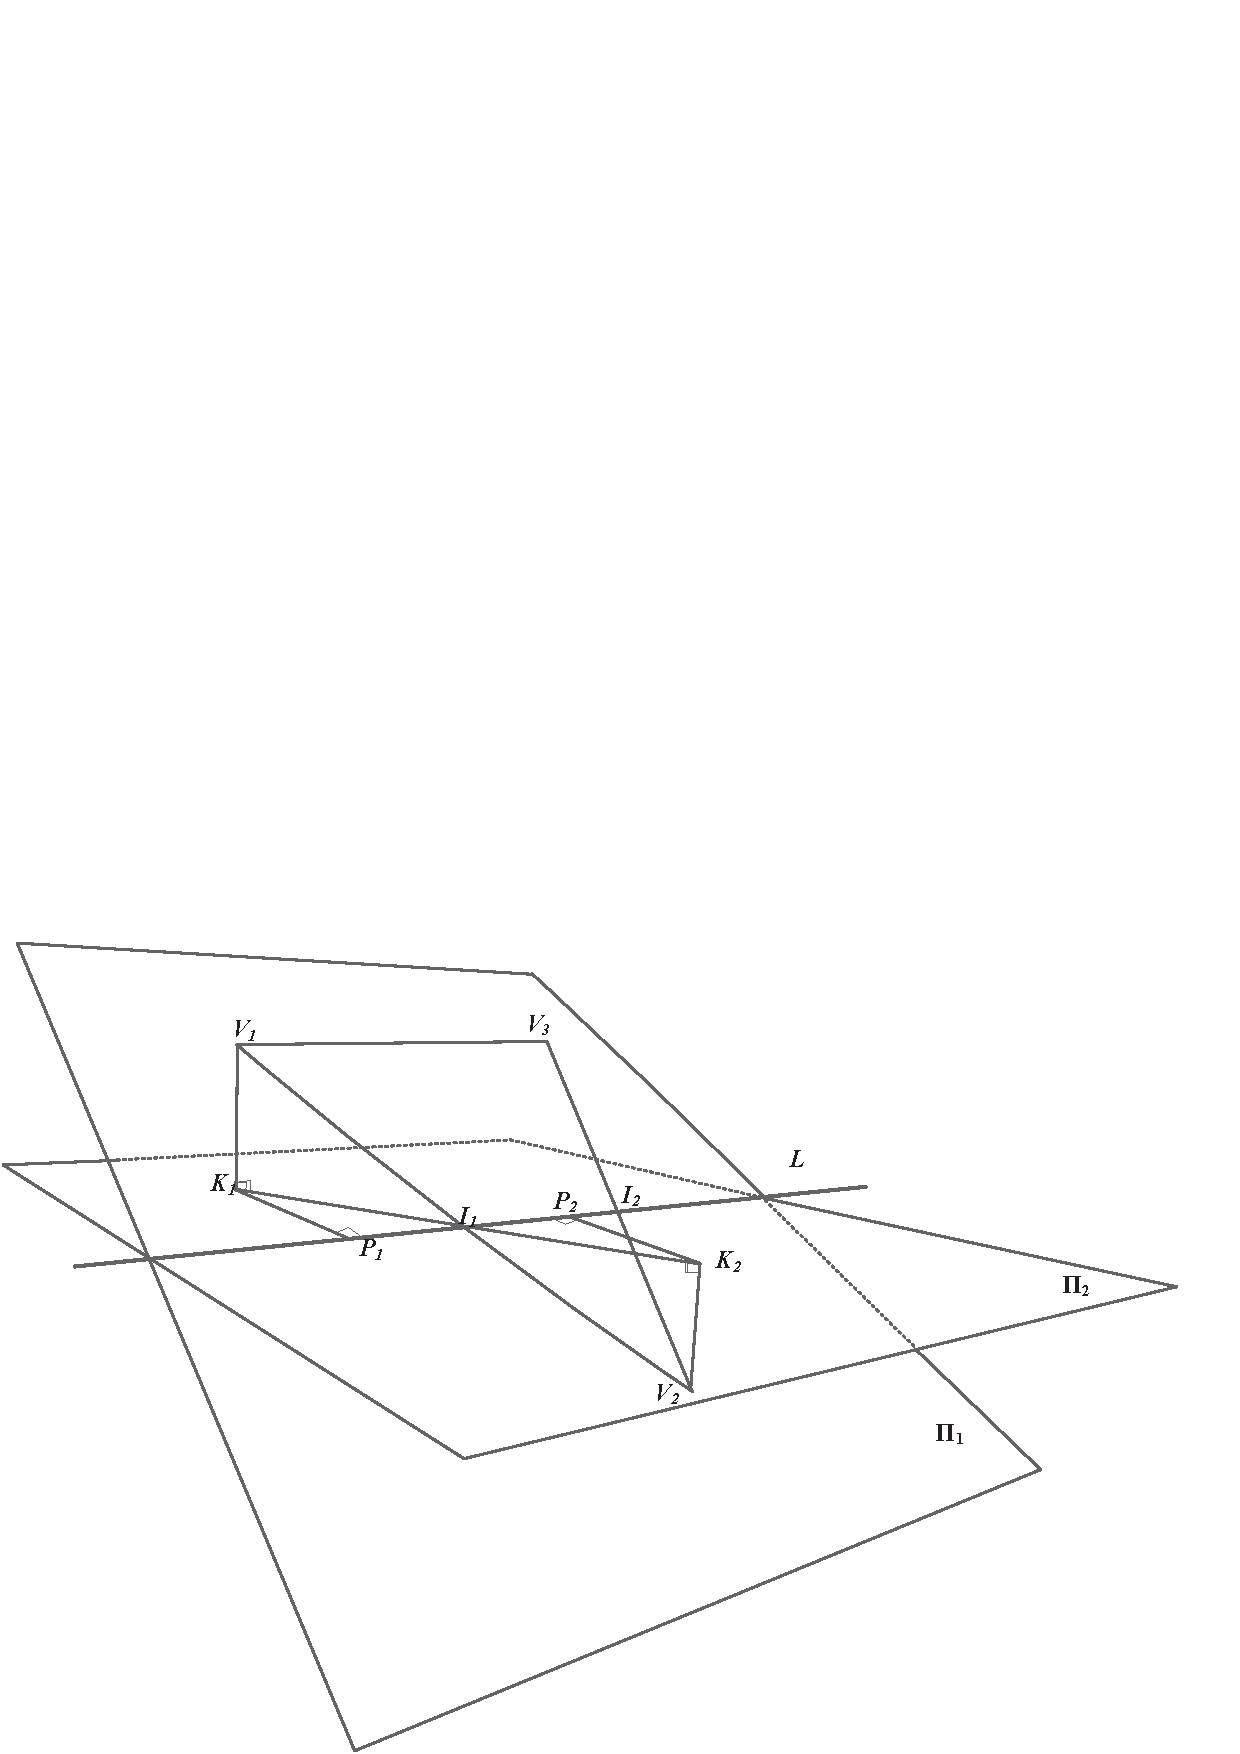
\includegraphics[width=4in]{TriangleTriangleTest2.pdf}
    \caption{求非共面三角形区间线段示意图\cite{Moller1997}}
  \label{fig:two:triangle:ui2}
\end{figure}

已知直线~$\bm{L}$~的方向为$\bm{n}_L = \bm{n}_1 \times \bm{n}_2$,设~$\bm{O}$~为~$\bm{L}$上一点,则直线的参数方程为
$\bm{L} = t \cdot \bm{n}_L + \bm{O}$,假设交点~$I_1 = t_1 \cdot \bm{n}_L + \bm{O}$,投影点满足
$p_1 = \bm{n}_L \cdot(\bm{V}_1 - \bm{O}), p_2 = \bm{n}_L \cdot (\bm{V}_2 - \bm{O})$,由图~\ref{fig:two:triangle:ui2}~可知,
$\bigtriangleup K_1P_1I_1 \sim \bigtriangleup K_2P_2I_1, \bigtriangleup V_1K_1I_1 \sim \bigtriangleup V_2K_2I_1$,可得

\begin{equation}
  \frac{t_1 - p_1}{p_2-p_1} = \frac{l_{11}}{l_{11}-l_{12}} \Rightarrow \newline
   t_1 = (p_2-p_1)\frac{l_{11}}{l_{11}-l_{12}} + p_1
  \label{equa:triangle:intersectionline:param}
\end{equation}

同理可得~$\bm{I}_2$~的参数~$t_2$,三角形~$T_2$~用相同的方法也能得到区间的参数,即可判断两个区间线段是否相交,进而可得该非共面的两个三角形是否相交。
完整的算法如~\ref{alg:triangles:intersection}~所示。

\begin{algorithm}[htbp]
\small
\caption{三角形求交算法}
\label{alg:triangles:intersection}
\begin{algorithmic}[1]
\Require
两个三角形的6个顶点 $T_1(\bm{U}_1, \bm{U}_2, \bm{U}_3), T_2(\bm{V}_1, \bm{V}_2, \bm{V}_3)$
\Ensure
是否相交

\Function{TriangleTriangleDetection}{$\bm{U}_1, \bm{U}_2, \bm{U}_3, \bm{V}_1, \bm{V}_2, \bm{V}_3$}
    \State {$\Pi_1 \gets \bm{n}_1 \cdot \bm{x}+d_1$} \Comment{按照公式~\ref{equa:tri:tri:plane}~计算$T_1$所在平面方程}
    \For {$i = 1 \to 3$}
        \State {$l_{1i} \gets \bm{n}_1 \cdot \bm{V}_i + d_1$} \Comment {计算$T_2$到$\Pi_1$的有向距离}
    \EndFor
    \If {$(l_{11} > 0 \textbf{~and~} l_{12} > 0 \textbf{~and~} l_{13} > 0) \textbf{or}
          (l_{11} < 0 \textbf{~and~} l_{12} < 0 \textbf{~and~} l_{13} < 0)$}
          \State \Return \textbf{False} \Comment{$T_2$在$\Pi_1$的同侧,排除}
    \EndIf
    \If {$l_{11} = 0 \textbf{~and~} l_{12} = 0 \textbf{~and~} l_{13} = 0$}
        \State \Return \Call{EdgeEdgeTest}{$\bm{U}_1, \bm{U}_2, \bm{U}_3, \bm{V}_1, \bm{V}_2, \bm{V}_3$}
        \State \Comment{$T_2$与$T_1$的共面,普通的边边相交测试}
    \EndIf
    \State {$\Pi_2 \gets \bm{n}_2 \cdot \bm{x}+d_2$} \Comment{按照公式~\ref{equa:tri:tri:plane}~计算$T_2$所在平面方程}
    \For {$i = 1 \to 3$}
        \State {$l_{2i} \gets \bm{n}_2 \cdot \bm{U}_i + d_2$} \Comment {计算$T_1$到$\Pi_2$的有向距离}
    \EndFor
    \If {$(l_{21} > 0 \textbf{~and~} l_{22} > 0 \textbf{~and~} l_{23} > 0) \textbf{or}
          (l_{21} < 0 \textbf{~and~} l_{22} < 0 \textbf{~and~} l_{23} < 0)$}
          \State \Return \textbf{False} \Comment{$T_1$在$\Pi_2$的同侧,排除}
    \EndIf
    \State {$t_1 \gets \Call{CalParam}{}, t_2 \gets \Call{CalParam}$}  
    \Comment {按照公式~\ref{equa:triangle:intersectionline:param}~计算线段$\bm{D}_1$的参数区间} 
    \State {$t_3 \gets \Call{CalParam}{}, t_4 \gets \Call{CalParam}$}  \Comment{类似的方法计算线段$\bm{D}_2$的参数区间} 
    \If {$\Call{Overlap}{t_1, t_2, t_3, t_4}$}
       \State \Return \textbf{True} \Comment{区间交叉,表明三角形相交返回\textbf{True}}
    \Else
       \State \Return \textbf{False}
    \EndIf
\EndFunction

\end{algorithmic}
\end{algorithm}

算法~\ref{alg:triangles:intersection}~第~10~行在进行边边测试子过程中,可通过点与有向线段的位置关系确定,如线段两个端点都在另外一个有向线段的一边说明两线段不相交,反之相交,不需要求解出实际的交点。
在实际实现过程中,往往需要引入容差以提高算法的稳定性。文献~\onlinecite{Moller1997}~介绍了更多的优化技巧。

\section{基于 $k$-CBP 的碰撞检测算法}
\label{sec:cd:baseon:kcbp}

凸包围多面体可应用于加速相关几何算法的整体效率, 图~\ref{lbl:bunny-box-kcbp-collsion-detection-example}
为利用~Bunny~模型进行碰撞检测的示例, 图中模型~1~与~2、2~与~3~的包围盒分别相交, 而其~$16$-CBP~仅~1~与~2~相交, 实际模型仅~1~与~2~相交.
用~$16$-CBP~可排除模型~2~与~3~之间的碰撞检测, 而仅用包围盒算法则无法排除, 显然检测模型~2~与~3~的~$16$-CBP~是否相交比直接通过检测模型~2~与~3~是否相交更省时间.
%在碰撞检测算法中, 在进行真实模型的相交检测前一般会用包围球、包围盒等包围体进行预先排除$^{[17]}$.

\subsection{静止场景中的碰撞检测算法}
\label{subsec:static:cd}

\begin{figure}[htbp] 
\centering
\includegraphics[width=5in]{bunny-box-kcbp-collsion-detection-example.png}
\caption{~$k-$CBP~应用于碰撞检测示例}
\label{lbl:bunny-box-kcbp-collsion-detection-example}
\end{figure}


模型的~$k$-CBP~相交后,会用模型的~AABB~树进一步对模型进行碰撞检测,模型的~AABB~树构造方法如第~\ref{subsec:kcbp:cd:aabb}~节所述,
图~\ref{fig:bunny:aabb:bvh:toplayer4}~是按照本文所采用的构造方法针对~Bunny~模型构造的~AABB~树形结构的顶上~4~层。

\begin{figure}[htpb]
  \centering
  \includegraphics[width=\textwidth]{bunny-aabb-bvh-4-layers.pdf}
  \caption{Bunny~模型的~AABB~树形结构(部分)}
  \label{fig:bunny:aabb:bvh:toplayer4}
\end{figure}

整体的碰撞检测算法流程图如图~\ref{fig:flowchart:cd}所示,首先扫描所有输入模型点集,对每个模型计算其包围盒,然后计算要参与碰撞检测的模型的包围盒对进行相交测试,
假设要计算参与碰撞检测的模型的包围盒相交的对数为~$n_1$,再对这~$n_1$~对模型计算其~$k$-CBP~并进行初始化,如构造~AABB~树、初始化~GJK~算法,并计算~$k$-CBP
是否相交,此步骤后剩余模型对数为~$n_2$,最后再对这~$n_2$~对模型进行构造~AABB~树进而进行相交测试,真实模型相交对数为~$n_3$。整个流程中,包围盒的命中率为$n_1 / n_3$,$k$-CBP~的命中率为~$n_2/n_3$。


\begin{figure}[htpb]
  \centering
  \includegraphics[width=\textwidth]{collision-detection-flowchart.pdf}
  \caption{碰撞检测算法流程图}
  \label{fig:flowchart:cd}
\end{figure}

\subsection{运动场景中的碰撞检测算法}
\label{subsec:moving:cd}

当在运动场景中的模型进行碰撞检测时,模型中的点坐标会更新,一种方法是重新计算模型中的所有点再对模型做碰撞检测,但当模型点数量较大时,此方法不可取;
另外一种算法是仍然利用静态场景中的~AABB~树形结构,仅重新计算将要碰撞的节点的坐标值,进而进行相交检测。
节点包围盒坐标在运动过程中发生变化,精确的包围盒是重新计算该节点包含原始模型的点在变化后的点坐标值的包围盒,本文利用一种近似算法即仅对包围盒的~8~个顶点进行转换
然后计算这8个顶点的包围盒,用这个近似包围盒进行遍历剪枝,当到叶子节点后,再重新计算网格模型的点的新坐标值用同样的方法进行相交检测。

模型围绕任意过原点的轴~$\bm{n}(x, y,
z)$~旋转任意角度~$\theta$~的变换矩阵如公式~\ref{equa:rotate:matrix}~所示,其中$\lambda
= 1-\cos\theta$,
详细的推导过程可以参考文献~\onlinecite{dunn20023d}。

\begin{equation}
%\small
\left\{
    \begin{array}{ll}
    \bm{R}(\bm{n},\theta) 
    &= 
          \cos\theta \begin{pmatrix}
                      1 & 0 & 0 \\
                      0 & 1 & 0 \\
                      0 & 0 & 1
                     \end{pmatrix}
          + \lambda \begin{pmatrix}
                    \bm{n}_x^2 & \bm{n}_x\bm{n}_y & \bm{n}_x\bm{n}_z \\
                    \bm{n}_x\bm{n}_y & \bm{n}_y^2 & \bm{n}_y\bm{n}_z \\
                    \bm{n}_x\bm{n}_z & \bm{n}_y\bm{n}_z & \bm{n}_z^2 
                    \end{pmatrix}
          + \sin\theta \begin{pmatrix}
                      0 & \bm{n}_z & -\bm{n}_y \\
                      -\bm{n}_z & 0 & \bm{n}_x \\
                      \bm{n}_y & -\bm{n}_x & 0
                      \end{pmatrix}
          \\
    ~&=  
        \begin{pmatrix}
            %\begin{array}{ccc}
              %\cos\theta+(1-\cos\theta)\cdot\bm{n}_x^2 & (1-\cos\theta)\cdot\bm{n}_x\cdot\bm{n}_y + \sin\theta\cdot\bm{n}_z & (1-\cos\theta)\cdot\bm{n}_x\cdot\bm{n}_z-\sin\theta\cdot\bm{n}_y \\
              %(1-\cos\theta)\cdot\bm{n}_x\cdot\bm{n}_y-\sin\theta\cdot\bm{n}_z & \cos\theta+(1-\cos\theta)\cdot\bm{n}_y^2 & (1-\cos\theta)\cdot\bm{n}_y\cdot\bm{n}_z+\sin\theta\cdot\bm{n}_x \\
              %(1-\cos\theta)\cdot\bm{n}_x\cdot\bm{n}_z + \sin\theta\cdot\bm{n}_y & (1-\cos\theta)\cdot\bm{n}_y\cdot\bm{n}_z - \sin\theta\cdot\bm{n}_x &  \cos\theta+(1-\cos\theta)\cdot\bm{n}_z^2 
              \cos\theta+\bm{n}_x^2\lambda & \bm{n}_x\bm{n}_y\lambda + \bm{n}_z\sin\theta & \bm{n}_x\bm{n}_z\lambda-\bm{n}_y\sin\theta \\
              \bm{n}_x\bm{n}_y\lambda - \bm{n}_z\sin\theta & \cos\theta+\lambda\bm{n}_y^2 & \bm{n}_y\bm{n}_z\lambda+\bm{n}_x\sin\theta \\
              \bm{n}_x\bm{n}_z\lambda + \bm{n}_y\sin\theta & \bm{n}_y\bm{n}_z\lambda - \bm{n}_x\sin\theta &  \cos\theta+\bm{n}_z^2\lambda 
          \end{pmatrix} \\
  \end{array}
\right.
\label{equa:rotate:matrix}
\end{equation}

当模型平移时,点~$\bm{P}(x, y, z)$~平移~$\bm{t}(t_x, t_y, t_z)$~后的点坐标为~$\bm{P}'(x+t_x, y+t_y, z+t_z)$,可用~$4 \times 4$~的变换矩阵~$\bm{T}$~表示,即
\begin{equation}
  \bm{T}(\bm{t}) =
  \begin{pmatrix}
    1 & 0 & 0 & t_x \\
    0 & 1 & 0 & t_y \\
    0 & 0 & 1 & t_z \\
    0 & 0 & 0 & 1 \\
  \end{pmatrix}
  \label{equa:translate:matrix}
\end{equation}

因此当模型平移旋转时产生的变换矩阵~$\bm{M}$~为
\begin{equation}
\bm{M}=\bm{R}(\bm{n}, \theta) \cdot \bm{T}(\bm{t}),
\label{equa:transform:matrix}
\end{equation}
AABB~节点包围盒更新后的算法如算法~\ref{alg:transform:box}~所示,
算法输入为平移向量$\bm{t}$及旋转方向和角度$\bm{n}, \theta$或者直接传入变化矩阵~$\bm{M}$~即可。

\begin{algorithm}[htbp]
\small
\caption{AABB节点包围盒更新算法}
\label{alg:transform:box}
\begin{algorithmic}[1]
\Require
AABB包围盒 $box$,
平移旋转变换矩阵$\bm{M}$
\Ensure
变换之后的包围盒 $box'$

\Function{TransformBox}{$box, \bm{M}$}
    \State $vertices \gets \Call{GetAABBVertices}{box}$ 
    \State $box' \gets \emptyset$
    \ForAll {$\bm{v} \in vertices$} \Comment{遍历~$box$~的8个顶点}
        \State {$\bm{v'}= \bm{M} \cdot \bm{v}$} \Comment{计算变换后的点坐标}
        \State $\Call{update}{box', \bm{v'}}$ \Comment{根据变换后的顶点~$\bm{v}$~更新$box'$}
    \EndFor
    \State \Return $box'$
\EndFunction
\end{algorithmic}
\end{algorithm}

运动场景中模型的碰撞检测算法如算法~\ref{alg:moving:cd}~所示,假设参与碰撞检测的两个模型中第一个运动且变换矩阵为~$\bm{M}$,第二个静止,
两个模型都运动时,可视第二个模型相对静止,将~$\bm{M}$~设置为第一个相对于第二个模型的相对变换矩阵。

\begin{algorithm}[htbp]
\small
\caption{运动场景中基于~AABB~树碰撞检测算法}
\label{alg:moving:cd}
\begin{algorithmic}[1]
\Require
两个模型~AABB~树的根节点 $root_0, root_1$ 及
平移旋转变换矩阵$\bm{M}$
\Ensure
模型是否相交 

\Function{MovingTraverseDetection}{$root_0, root_1, \bm{M}$}
    \State $mBox \gets \Call{TransformBox}{\bm{M}, root_0.box} $ \Comment{按照算法~\ref{alg:transform:box}~计算运动后的包围盒}
    \State $c \gets \Call{Intersect}{mBox, root_1.box} $
    \If {$c = \textbf{False}$}
        \State \Return \textbf{False} \Comment{包围盒不相交,直接返回\textbf{False}}
    \EndIf
    \If {$root_0.\Call{IsLeaf}$}
        \If {$root_1.\Call{IsLeaf}$} \Comment{两个叶子节点的原始几何进行相交测试} 
              \ForAll {$p_1 \in root_0.primitives$}
                  \ForAll {$p_2 \in root_1.primitives$}
                  \State \Return {$\Call{Intersect}{\bm{M}, p_1, p_2}$} \Comment{将$\bm{p}_1$应用于变换矩阵$\bm{M}$后采用算法\ref{sec:intersection:triangles}中进行三角网格相交测试}
                  \EndFor
              \EndFor 
        \Else
            \If {$\Call{MovingTraverseDetection}{root_0, root_1.left} \hspace{0.5em} \textbf{or} \newline \hspace{4em}
                \hspace*{5.5em} \Call{MovingTraverseDetection}{root_0, root_1.right}$} \hspace{2em}
                \State \Return \textbf{True}
            \EndIf
        \EndIf
    \Else
        \If {$root_1.\Call{IsLeaf}$}
            \If {$\Call{MovingTraverseDetection}{root_0.left, root_1} \hspace{0.5em} \textbf{or} \newline \hspace{4em}
                 \hspace*{5.5em} \Call{MovingTraverseDetection}{root_0.right, root_1}$}
            \State \Return \textbf{True}
            \EndIf
        \Else \Comment{两个节点都有孩子节点}
            \If {$\Call{MovingTraverseDetection}{root_0.left, root_1.left}  \hspace{0.5em} \textbf{or} \newline \hspace{4em}
                 \hspace*{5.5em} \Call{MovingTraverseDetection}{root_0.left, root_1.right} \hspace{0.5em} \textbf{or} \newline \hspace{4em}
                 \hspace*{5.5em} \Call{MovingTraverseDetection}{root_0.right, root_1.left} \hspace{0.5em} \textbf{or} \newline \hspace{4em}
                 \hspace*{5.5em} \Call{MovingTraverseDetection}{root_0.right, root_1.right}$}
                 \State \Return \textbf{True}
            \EndIf
      \EndIf
    \EndIf
    \State \Return \textbf{False}
\EndFunction
\end{algorithmic}
\end{algorithm}

算法~\ref{alg:moving:cd}~是一个递归算法,从~AABB~树的根节点起向底层进行深度优先遍历,当检测到运动后的模型的某两个叶子节点的包围盒相交时,遍历其三角网格的相交检测算法,在实际实现过程中,本文的叶子节点仅含一个三角网格。
运动模型的三角网格应用变换矩阵得到一个新的三角网格,同样用~\ref{sec:intersection:triangles}~的算法对新的三角网格进行相交测试。
除了用该递归算法外,也可对算法~\ref{alg:aabbtree:traverse:iterator}~进行稍许改动(只需改变包围盒检测和三角网格检测的函数)的迭代算法,此处不在赘述。

\section{实验结果}
\label{sec:exper-cd}

\subsection{与包围盒过滤算法对比}
\label{subsec:exper:box:kcbp}

本文实验通过生成不同数量的模型(模型位置和旋转角度随机生成), 碰撞检测时首先判断包围盒是否相交, 然后判断凸包围多面体是否相交, 最后再判断实际模型是否相交.
凸包围多面体之间的碰撞检测时可采用文献~${[27]}$~中提到的方法,
本文案例中模型和凸包围多面体是否相交都采用了普通~AABB~树的方式进行判断,
从如表~\ref{tab:exp:box:kcbp:collsiondetection}~的实验结果可看出含有凸包多围体的模型之间的碰撞检测算法能显著提高整体应用的效率. 

%\begin{landscape} 横放,效果不好看, 还是将表头的单位去掉了
\begin{table}[htbp]
\caption{$k$-CBP~和包围盒应用于碰撞检测结果对比}
\label{tab:exp:box:kcbp:collsiondetection}
\centering
\begin{tabular}{lccccccl}
 \toprule[1.5pt]
  n& c(Box) & c($16$-CBP) &  t(Box) & t($16$-CBP) & r(Box) & r($k$-CBP) & n(Model) \\
  \midrule[1.0pt]
%  10 & 0.1 & 1.8 & 26.0  & 0.1 & 2 & 0 & 0\\
%  30 & 0.2 & 2.9 & 134.0  & 70.0 & 11 & 6 & 5\\
%  50 & 0.5 & 4.8 & 506.0  & 255.2 & 41 & 22 & 19 \\
%  70 & 0.4 & 4.8 & 901.1  & 492.5 & 77 & 42 & 34 \\
%  90 & 0.7 & 5.7 & 1324.0  & 734.7 & 110 & 63 & 46 \\
%  100 & 0.7 & 7.8 & 1481.0  & 870.7 & 127 & 73 & 55 \\
%  150 & 1.0 & 9.8 & 4153.1  & 2473.0 & 349 & 212 & 150 \\
%  200 & 1.6 & 12.8 & 8049.3 & 4430.9 & 685 & 394 & 281 \\
   10 & 0.1 & 1.8 &    26.0  & 0.1    & 0.00  & 100.00 & 0\\
   30 & 0.2 & 2.9 &   134.0  & 70.0   & 45.45 & 83.33 & 5\\
   50 & 0.5 & 4.8 &   506.0  & 255.2  & 46.34 & 86.36 & 19 \\
   70 & 0.4 & 4.8 &   901.1  & 492.5  & 44.16 & 80.95 & 34 \\
   90 & 0.7 & 5.7 &  1324.0  & 734.7  & 41.82 & 73.02 & 46 \\
  100 & 0.7 & 7.8 &  1481.0  & 870.7  & 43.31 & 75.34 & 55 \\
  150 & 1.0 & 9.8 &  4153.1  & 2473.0 & 42.98 & 70.75 & 150 \\
  200 & 1.6 & 12.8 & 8049.3  & 4430.9 & 41.02 & 71.32 & 281 \\
  \bottomrule[1.5pt]
 \end{tabular}
\end{table}
%\end{landscape}

如表~\ref{tab:exp:box:kcbp:collsiondetection}~所示,
其中~n~表示场景中模型的数量, c(Box), c($16$-CBP)分别表示模型包围盒的构造时间和凸包围16面体的构造时间(单位ms)\footnote{此处的时间为得到一个$k$-CBP后直接通过应用变换矩阵得到新的$k$-CBP总时间且是利用~GPU~搜索截面的时间,后文与~$k$-DOP对比均采用~CPU~算法实现}, t(Box), t($16$-CBP)~分表表示用包围盒进行碰撞检测和利用凸包围16面体进行碰撞检测所耗费的时间,
其中~r(Box), r($16$-CBP)分别表示包围盒、16-CBP~的命中率(即用实际模型相交的数量除以包围体检测出来相交的数量), ~n(Model)模型实际相交的数量, 显然计算模型包围盒所耗费的时间要明显少于计算凸包围多面体的时间, 但由于凸包围多面体比包围盒紧致,
因而命中率比包围盒高, 能排除更多本不相交的模型进而节省碰撞检测总时间, 提高算法效率。该部分工作已经发表,详细内容见参考文献~\onlinecite{tanglei2014}。

\subsection{静止场景中与~$k$-DOP~算法对比}
\label{subsec:exper:kdop:kcbp:static}

为了和K-DOP进行对比,相同模型,kcbp也与kdop一样扫描点击重新构造,且都是用CPU实现的算法。


\subsection{运动场景中与~$k$-DOP~算法对比}
\label{subsec:exper:kdop:kcbp:dynamic}

为了和K-DOP进行对比,相同模型,kcbp也与kdop一样扫描点击重新构造,且都是用CPU实现的算法。


%%% Local Variables: 
%%% mode: latex
%%% TeX-master: t
%%% End: 

\chapter{总结与展望}
\label{cha:kcbp-collision-detection}
算法基本概念及框架

\section{总结}
\label{sec:gen-normals}

\section{展望}
\label{sec:search-planes}



%%% 其它部分
\backmatter

% 本科生要这几个索引,研究生不要。选择性留下。
\makeatletter
\ifthu@bachelor
  % 插图索引
  \listoffigures
  % 表格索引
  \listoftables
  % 公式索引
  %\listofequations
\fi
\makeatother


% 参考文献
\bibliographystyle{thubib}
\bibliography{ref/chinese-ref,ref/papers-bib-in-google}


% 致谢
%%% Local Variables:
%%% mode: latex
%%% TeX-master: "../main"
%%% End:

\begin{ack}

  衷心感谢我的导师 雍俊海 教授 对本人学习及工作的精心指导。
  雍老师工作勤奋、治学严谨令我非常敬佩,他严谨的学术精神以及勤奋忘我的工作态度给我留下了深刻的印象,让我终生难忘。
  
  感谢施侃乐老师对本人的指导和帮助,GEMS~8~研发团队在本人求学过程中的提供了不少关心和帮助,特此表示衷心感谢。

  感谢家人的理解和支持。

\end{ack}


% 附录
%\begin{appendix}
%%%% Local Variables: 
%%% mode: latex
%%% TeX-master: "../main"
%%% End: 
\chapter{基于着色器的并行算法关键代码}
\label{appendix:shader-chapter}

\section{基于深度缓冲的算法}
\label{app-sec:shader-z-buffer}

%\lstinputlisting[language={shader}, caption={Vertex shader(Z buffer algorithm)}, label=vertex_shader_zbuffer]{shader_zbuffer.vert}
\lstinputlisting[language={shader}]{shader_zbuffer.vert}

\lstinputlisting[language={shader}]{shader_zbuffer.frag}


\section{基于乒乓技术的算法}
\label{app-sec:shader-rtt-pingpong}

\lstinputlisting[language={shader}]{shader_rrt_pingpong.frag}

%\end{appendix}

% 个人简历
\begin{resume}

  \resumeitem{个人简历}

  1989 年 12 月 30 日出生于 重庆市石柱土家族自治县。
  
  2008 年 9 月考入 中南 大学 软件学院 软件工程专业,2012 年 7 月本科毕业并获得工学学士学位。
  
  2012 年 9 月免试进入清华大学软件学院攻读工学硕士学位至今。

  \resumeitem{发表的学术论文} % 发表的和录用的合在一起

  \begin{enumerate}[{[}1{]}]
    \item \textbf{唐磊}, 李春平, 杨柳. 统计策略序列模式挖掘及其在软件缺陷预测中的应用. 计算机科学, 2013, 40(5): 164-167.
    \item Shi KanLe, Yong JunHai, \textbf{Tang Lei}, et al. Polar NURBS surface with curvature continuity, Computer Graphics Forum. 2013, 32(7): 363-370.
    \item \textbf{唐磊}, 施侃乐, 雍俊海等. 模型适应的凸包围多面体并行生成算法. 中国科学:信息科学, 2014, 44(12): 1515-1526.
    \item 林建立, \textbf{唐磊}, 雍俊海等.多边形网格的非流形封闭三角形网格正则化. 计算机辅助设计与图形学学报,2014,26(10):1557-1566.
  \end{enumerate}

%  \resumeitem{研究成果} % 有就写,没有就删除
%  \begin{enumerate}[{[}1{]}]
%  \item 任天令, 杨轶, 朱一平, 等. 硅基铁电微声学传感器畴极化区域控制和电极连接的
%    方法: 中国, CN1602118A. (中国专利公开号.)
%  \item Ren T L, Yang Y, Zhu Y P, et al. Piezoelectric micro acoustic sensor
%    based on ferroelectric materials: USA, No.11/215, 102. (美国发明专利申请号.)
%  \end{enumerate}

\end{resume}

\end{document}
